
\documentclass[12pt,a4paper]{article}

\usepackage[utf8]{inputenc}
\usepackage[T1]{fontenc}
\usepackage[brazil]{babel}
\usepackage{geometry}
\usepackage{graphicx}
\usepackage{booktabs}
\usepackage{longtable}
\usepackage{array}
\usepackage{float}
\usepackage{caption}
\usepackage{subcaption}
\usepackage{amsmath}
\usepackage{hyperref}
\usepackage{xcolor}

\geometry{left=2.5cm,right=2.5cm,top=2.5cm,bottom=2.5cm}
\graphicspath{{../}}
\hypersetup{colorlinks=true, linkcolor=blue, urlcolor=blue, citecolor=blue}

\title{Implementação e Avaliação do ClonalG para Agrupamento de Dados}
\author{Vinicius Macedo Colares Botelho (vmcb) \\ Marcos Daniel Maia Marques (lmrc) \\ Computação Natural -- Segundo Trabalho Prático}
\date{Maio de 2026}

\begin{document}
\maketitle

\begin{abstract}
Este relatório apresenta a implementação e avaliação do algoritmo de seleção clonal ClonalG aplicado ao problema de agrupamento de dados. O objetivo foi investigar a capacidade de uma abordagem bioinspirada de organizar dados multidimensionais e compará-la com o algoritmo clássico k-Means. Foram utilizados cinco conjuntos de dados fornecidos para o trabalho, submetidos a uma etapa de limpeza, imputação, normalização, análise exploratória, ajuste de parâmetros, descoberta do número de grupos e comparação por meio do índice Silhouette. Os resultados mostram que o ClonalG obteve desempenho competitivo com o k-Means, empatando nos conjuntos mais estruturados, superando-o no DataSet 4 e ficando levemente abaixo nos DataSets 2 e 3 na configuração avaliada.
\end{abstract}

\tableofcontents
\newpage

\section{Introdução}
O agrupamento de dados é uma tarefa de aprendizado não supervisionado cujo objetivo é particionar observações em grupos coerentes, de forma que elementos pertencentes ao mesmo grupo sejam mais semelhantes entre si do que em relação aos demais grupos. Essa tarefa é importante em problemas de reconhecimento de padrões, mineração de dados, segmentação e análise exploratória.

Neste trabalho foi implementado o algoritmo ClonalG, inspirado no princípio de seleção clonal do sistema imunológico artificial. A ideia central é manter uma população de anticorpos candidatos, avaliar sua afinidade com o problema, proliferar os melhores candidatos, aplicar hipermutação somática e preservar uma memória populacional de soluções de maior qualidade. No contexto de agrupamento, cada anticorpo representa um conjunto de centroides, e a qualidade da solução é medida pelo índice Silhouette.

O algoritmo ClonalG foi comparado diretamente ao k-Means da biblioteca Scikit-Learn. O k-Means é uma referência clássica para particionamento baseado em centroides, mas depende fortemente da escolha de \(k\), da inicialização e da geometria dos dados. Já o ClonalG permite explorar o espaço de soluções por mutação e substituição populacional, oferecendo uma alternativa estocástica para escapar de configurações locais inadequadas.

\section{Materiais e Métodos}

\subsection{Conjuntos de dados}
Foram utilizados os cinco conjuntos de dados disponibilizados para o trabalho. Os arquivos originais estavam no diretório \texttt{datasets/}. Durante a verificação do projeto, foi identificado que os CSVs continham uma coluna de índice exportada pelo pandas. Essa coluna foi removida antes da normalização para evitar que um atributo artificial interferisse na distância euclidiana, no Silhouette, no ClonalG e no k-Means.

A Tabela~\ref{tab:dados} resume as dimensões após a correção do pré-processamento.

\begin{table}[H]
\centering
\caption{Resumo dos conjuntos de dados após remoção da coluna de índice.}
\label{tab:dados}
\begin{tabular}{cccc}
\toprule
DataSet & Amostras & Atributos reais & Valores ausentes \\
\midrule
1 & 300 & 2 & 0 \\
2 & 1010 & 2 & 0 \\
3 & 300 & 4 & 0 \\
4 & 230 & 2 & 0 \\
5 & 440 & 6 & 0 \\
\bottomrule
\end{tabular}
\end{table}

\subsection{Pré-processamento}
O pré-processamento foi implementado no script \texttt{preprocessamento.py}. As etapas realizadas foram:

\begin{enumerate}
    \item leitura dos cinco arquivos CSV;
    \item detecção e remoção de colunas de índice exportadas;
    \item conversão dos atributos para formato numérico;
    \item imputação por média quando necessário;
    \item padronização com \texttt{StandardScaler};
    \item geração dos arquivos \texttt{DataSet\textit{i}\_scaled.csv};
    \item geração de gráficos exploratórios em 2D ou PCA 2D.
\end{enumerate}

A normalização é necessária porque tanto o ClonalG quanto o k-Means usam distâncias euclidianas. Sem essa etapa, atributos com maior escala numérica dominariam a avaliação de similaridade.

\subsection{Visualização exploratória}
Para conjuntos com dois atributos, os gráficos foram gerados diretamente no plano original. Para conjuntos com mais de dois atributos, foi utilizada PCA com duas componentes apenas para visualização. A PCA não altera os dados usados no treinamento ou no cálculo do Silhouette; ela apenas permite representar os agrupamentos em duas dimensões.

\begin{figure}[H]
\centering
\begin{subfigure}{0.48\textwidth}
\centering
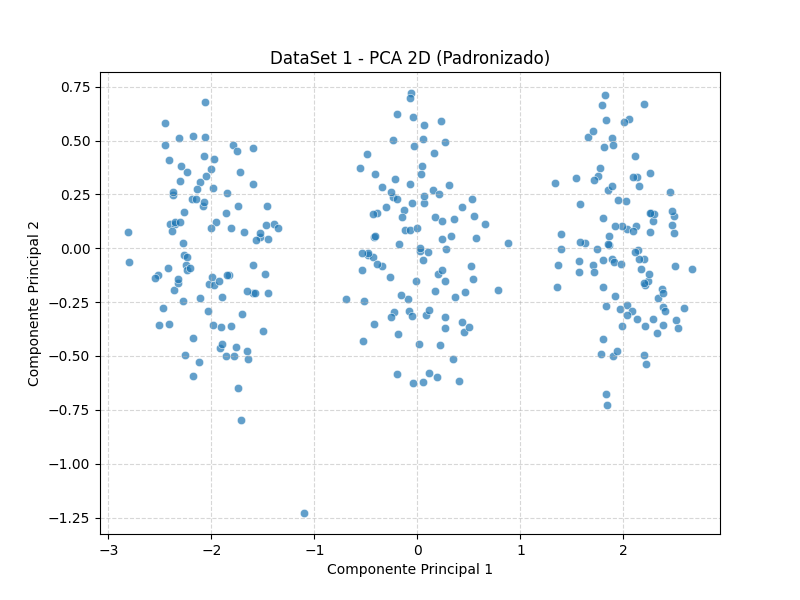
\includegraphics[width=\textwidth]{resultados/etapa1/dataset1_plot.png}
\caption{DataSet 1}
\end{subfigure}
\begin{subfigure}{0.48\textwidth}
\centering
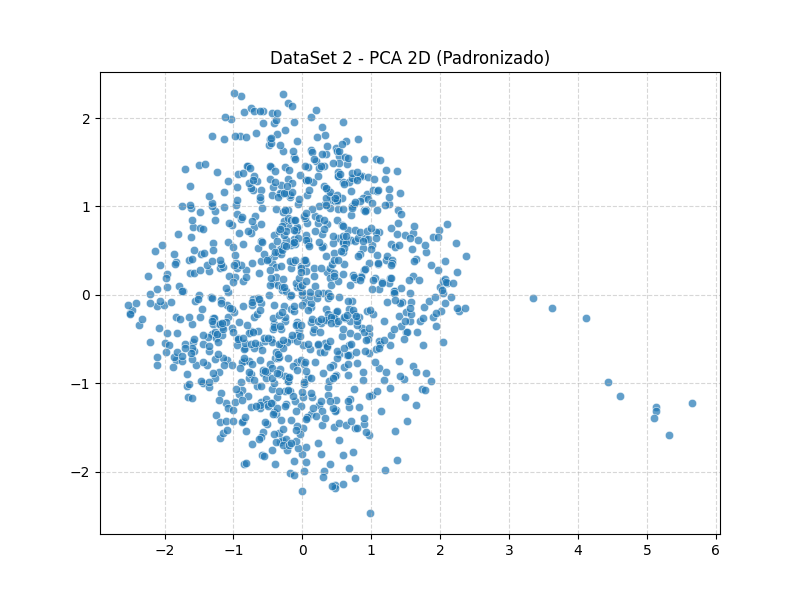
\includegraphics[width=\textwidth]{resultados/etapa1/dataset2_plot.png}
\caption{DataSet 2}
\end{subfigure}

\begin{subfigure}{0.48\textwidth}
\centering
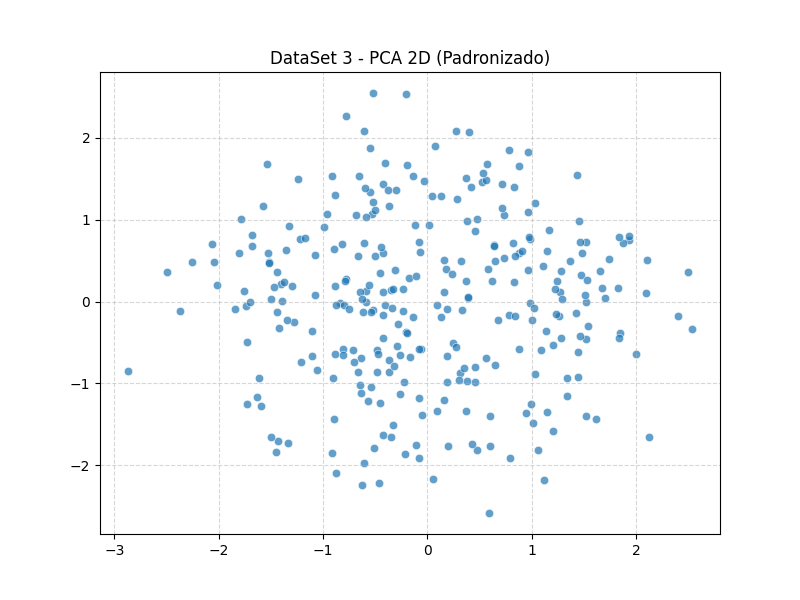
\includegraphics[width=\textwidth]{resultados/etapa1/dataset3_plot.png}
\caption{DataSet 3}
\end{subfigure}
\begin{subfigure}{0.48\textwidth}
\centering
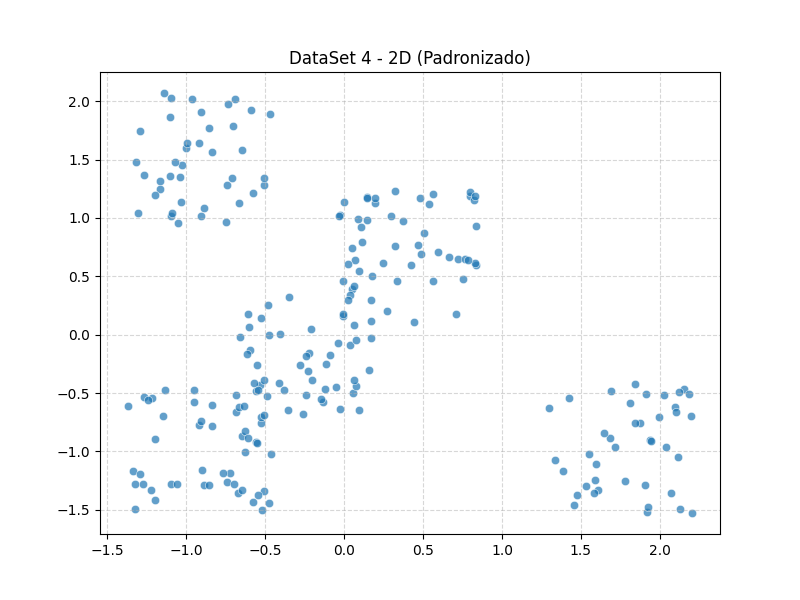
\includegraphics[width=\textwidth]{resultados/etapa1/dataset4_plot.png}
\caption{DataSet 4}
\end{subfigure}

\begin{subfigure}{0.55\textwidth}
\centering
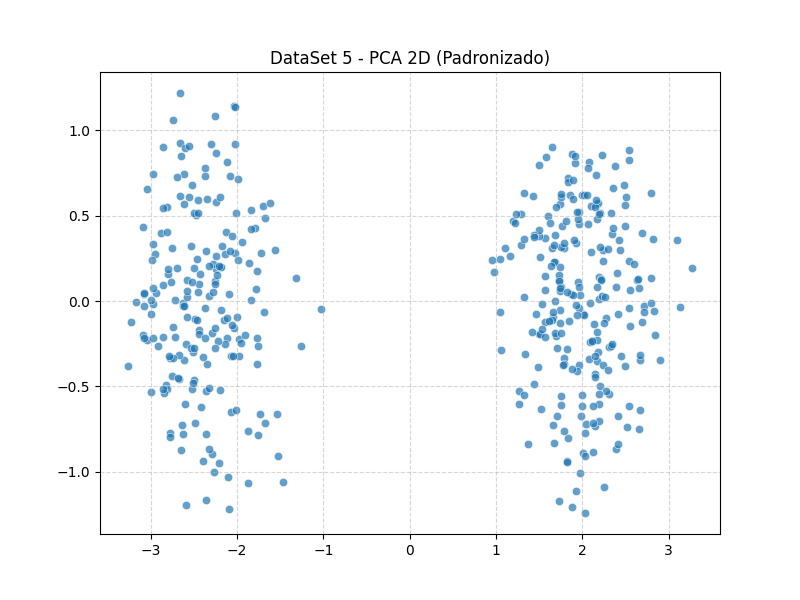
\includegraphics[width=\textwidth]{resultados/etapa1/dataset5_plot.png}
\caption{DataSet 5}
\end{subfigure}
\caption{Análise exploratória dos cinco datasets após padronização.}
\label{fig:eda}
\end{figure}

\subsection{Representação da solução}
No ClonalG implementado, cada anticorpo representa uma solução candidata de agrupamento. Formalmente, um anticorpo \(A\) é uma matriz de centroides:

\[
A = \{c_1, c_2, \ldots, c_k\}, \quad c_j \in \mathbb{R}^d
\]

em que \(k\) é o número de grupos e \(d\) é a dimensionalidade dos dados. Para atribuir cada amostra a um grupo, calcula-se a distância euclidiana entre a amostra e todos os centroides do anticorpo, escolhendo o centroide mais próximo.

\subsection{Função de afinidade}
A afinidade foi medida pelo índice Silhouette, que avalia simultaneamente coesão intragrupo e separação intergrupos. Para uma amostra \(i\), o Silhouette é definido por:

\[
s(i) = \frac{b(i) - a(i)}{\max(a(i), b(i))}
\]

em que \(a(i)\) é a distância média da amostra aos elementos do próprio grupo e \(b(i)\) é a menor distância média da amostra aos elementos de outro grupo. O valor final é a média de \(s(i)\) para todas as amostras. Valores próximos de 1 indicam agrupamentos mais bem separados; valores próximos de 0 indicam fronteiras pouco definidas; valores negativos sugerem atribuições inadequadas.

Na afinidade interna do ClonalG, foi adotada uma amostragem de Silhouette para reduzir custo computacional em datasets maiores. A avaliação final e as tabelas comparativas usam o Silhouette completo.

\subsection{Processos imunológicos implementados}
Os quatro processos exigidos no enunciado foram implementados:

\begin{itemize}
    \item \textbf{Reconhecimento}: cada anticorpo gera rótulos por distância euclidiana aos centroides, e sua afinidade é avaliada pelo Silhouette.
    \item \textbf{Proliferação}: anticorpos de maior afinidade produzem mais clones. O número de clones é proporcional à afinidade normalizada.
    \item \textbf{Variação}: os clones sofrem hipermutação somática com intensidade inversamente proporcional à afinidade. Quanto menor a afinidade, maior a perturbação aplicada aos centroides.
    \item \textbf{Seleção e diversidade}: os melhores anticorpos e clones são preservados na memória populacional. Uma parcela dos piores indivíduos é substituída por novos anticorpos aleatórios para manter diversidade.
\end{itemize}

A taxa de seleção foi separada da taxa de substituição. A variável \texttt{selection\_rate} controla a porcentagem dos melhores anticorpos usados na etapa de clonagem, enquanto \texttt{replace\_rate} controla a substituição dos piores indivíduos ao fim da geração.

\subsection{Pseudocódigo do ClonalG}
\begin{verbatim}
Entrada: dados X, faixa ou valor de k, N anticorpos, rho, beta,
         taxa de seleção, taxa de substituição, número de gerações
Saída: melhor anticorpo A*

Inicializar população P com N anticorpos aleatórios
Para cada geração t:
    Para cada anticorpo A em P:
        Atribuir cada amostra ao centroide mais próximo de A
        Calcular afinidade(A) pelo índice Silhouette
    Normalizar afinidades
    Selecionar os melhores anticorpos conforme taxa de seleção
    Para cada anticorpo selecionado:
        Gerar número de clones proporcional à afinidade
        Para cada clone:
            Aplicar ruído gaussiano com intensidade exp(-rho * afinidade)
            Opcionalmente adicionar ou remover centroides se k for variável
    Avaliar clones pelo Silhouette
    Combinar população original e clones
    Preservar os N melhores indivíduos como memória populacional
    Substituir uma fração dos piores por anticorpos aleatórios
Retornar o melhor anticorpo encontrado
\end{verbatim}

\subsection{Ajuste de parâmetros}
Foi implementado um algoritmo de busca em grade no script \texttt{experimentos\_parametros.py}. A busca avaliou diferentes configurações do ClonalG e comparou os resultados com o k-Means. Os parâmetros testados foram:

\begin{itemize}
    \item número de anticorpos: \(10\) e \(20\);
    \item fator de mutação \(\rho\): \(1.0\) e \(2.5\);
    \item fator de clonagem \(\beta\): \(10\);
    \item taxa de substituição: \(0.05\) e \(0.20\);
    \item taxa de seleção: \(0.50\) e \(0.85\);
    \item valores de \(k\) candidatos obtidos a partir da avaliação do k-Means para \(k \in \{2,3,4,5,6\}\).
\end{itemize}

A busca inicial executou uma repetição por configuração para reduzir tempo de execução. As melhores configurações foram reavaliadas com três repetições. Esse desenho experimental é suficiente para comparar tendências, mas pode ser expandido aumentando as constantes \texttt{SEARCH\_RUNS}, \texttt{VALIDATION\_RUNS}, \texttt{N\_ITERATIONS} e a grade de parâmetros.

\section{Resultados}

\subsection{Melhores configurações encontradas}
A Tabela~\ref{tab:melhores} apresenta as melhores configurações validadas para cada dataset, comparadas ao k-Means com o mesmo valor de \(k\).

\begin{table}[H]
\centering
\caption{Melhores configurações validadas do ClonalG e comparação com k-Means.}
\label{tab:melhores}
\resizebox{\textwidth}{!}{%
\begin{tabular}{cccccccccc}
\toprule
DS & k & N & \(\rho\) & \(\beta\) & Subst. & Sel. & ClonalG médio & k-Means & Delta \\
\midrule
1 & 3 & 10 & 1.0 & 10 & 0.05 & 0.50 & 0.6480 & 0.6480 & 0.0000 \\
2 & 5 & 20 & 1.0 & 10 & 0.20 & 0.50 & 0.3973 & 0.4185 & -0.0212 \\
3 & 6 & 20 & 2.5 & 10 & 0.20 & 0.85 & 0.2153 & 0.2221 & -0.0068 \\
4 & 4 & 10 & 1.0 & 10 & 0.05 & 0.50 & 0.5905 & 0.5866 & 0.0040 \\
5 & 2 & 10 & 1.0 & 10 & 0.05 & 0.85 & 0.6644 & 0.6644 & 0.0000 \\
\bottomrule
\end{tabular}%
}
\end{table}

\subsection{Comparação final ClonalG vs k-Means}
Após a busca, o comparativo final foi reexecutado com as melhores configurações. O ClonalG foi executado três vezes por dataset, registrando média, desvio padrão e melhor execução. O k-Means foi executado com \texttt{n\_init=30} e semente fixa.

\begin{table}[H]
\centering
\caption{Comparação final usando as melhores configurações do ClonalG.}
\label{tab:comparativo-final}
\resizebox{\textwidth}{!}{%
\begin{tabular}{cccccccc}
\toprule
DS & k & ClonalG média & Desvio & Melhor ClonalG & k-Means & Delta médio & Interpretação \\
\midrule
1 & 3 & 0.6480 & 0.0000 & 0.6480 & 0.6480 & 0.0000 & Empate \\
2 & 5 & 0.4082 & 0.0038 & 0.4109 & 0.4185 & -0.0104 & k-Means superior \\
3 & 6 & 0.2214 & 0.0005 & 0.2220 & 0.2221 & -0.0007 & Empate técnico \\
4 & 4 & 0.5905 & 0.0000 & 0.5905 & 0.5866 & 0.0040 & ClonalG superior \\
5 & 2 & 0.6644 & 0.0000 & 0.6644 & 0.6644 & 0.0000 & Empate \\
\bottomrule
\end{tabular}%
}
\end{table}

\begin{figure}[H]
\centering
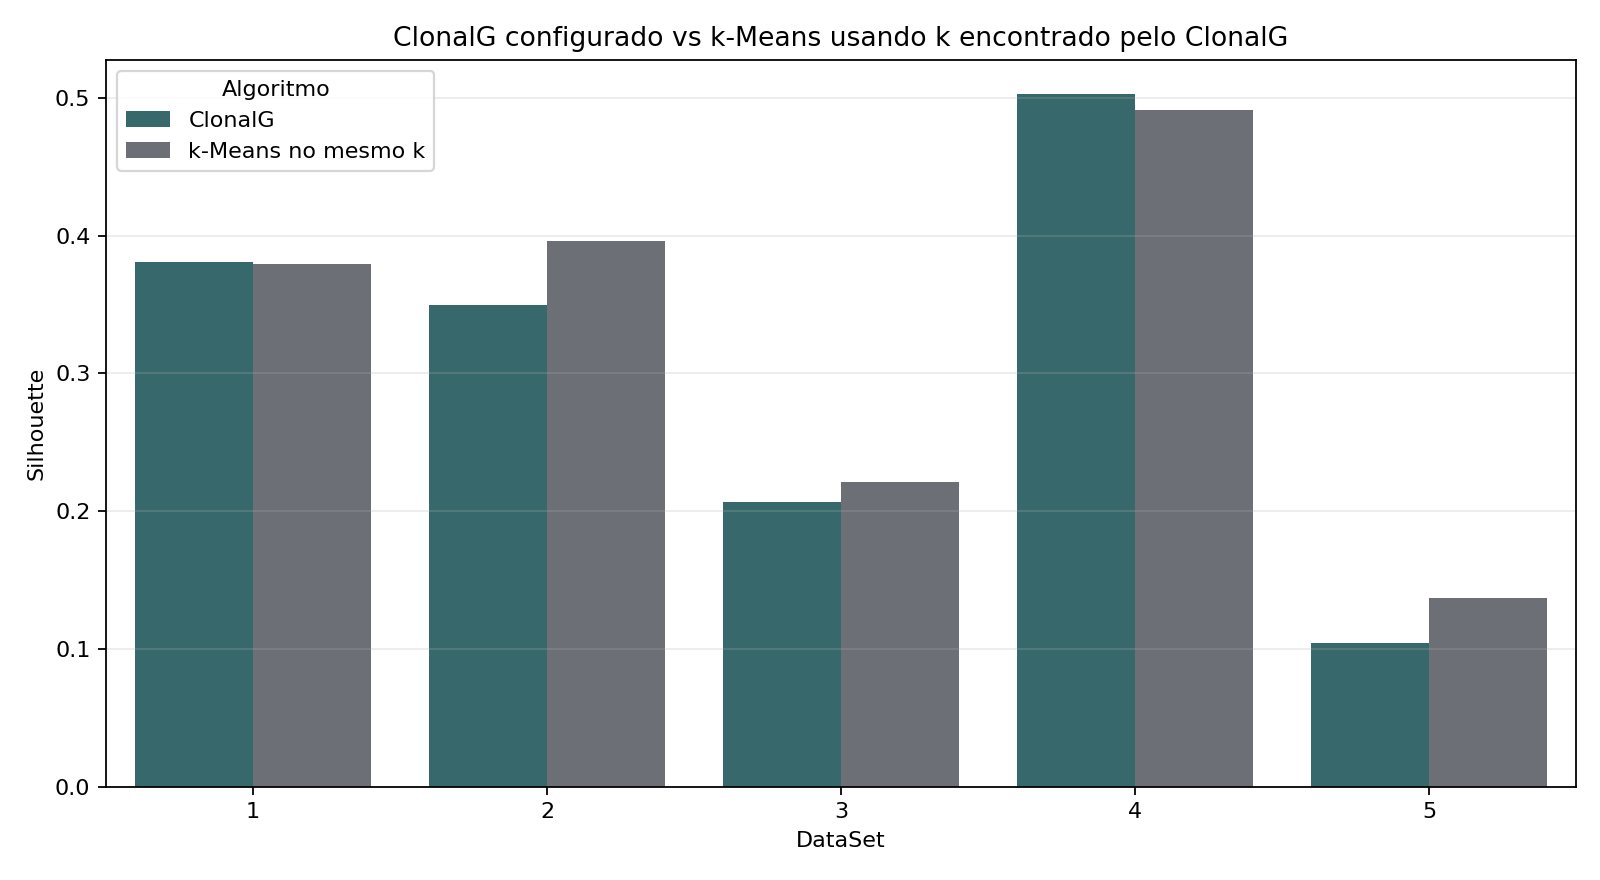
\includegraphics[width=0.85\textwidth]{resultados/etapa3_parametros/comparativo_melhores_vs_kmeans.png}
\caption{Comparação agregada entre melhores configurações do ClonalG e k-Means.}
\label{fig:comparativo-agregado}
\end{figure}

\subsection{Descoberta automática do número de clusters}
Também foi avaliada a capacidade do ClonalG de operar com \(k\) variável. Nessa versão, os anticorpos podem adicionar ou remover centroides durante a mutação estrutural, dentro da faixa definida. A Tabela~\ref{tab:k-auto} apresenta os valores encontrados.

\begin{table}[H]
\centering
\caption{Descoberta automática de \(k\) pelo ClonalG.}
\label{tab:k-auto}
\begin{tabular}{ccc}
\toprule
DataSet & k descoberto & Melhor Silhouette \\
\midrule
1 & 3 & 0.6480 \\
2 & 5 & 0.4215 \\
3 & 5 & 0.2250 \\
4 & 4 & 0.5905 \\
5 & 2 & 0.6615 \\
\bottomrule
\end{tabular}
\end{table}

Os valores de \(k\) encontrados são coerentes com os melhores valores obtidos pelo k-Means em vários datasets. Isso indica que a mutação estrutural contribuiu para explorar diferentes complexidades de modelo, ainda que o critério de decisão continue baseado no Silhouette.

\subsection{Evolução do Silhouette}
Os gráficos de evolução mostram a melhora progressiva da afinidade durante as gerações. Como o ClonalG preserva os melhores anticorpos, a curva tende a se estabilizar quando a população encontra uma configuração de centroides de alta afinidade.

\begin{figure}[H]
\centering
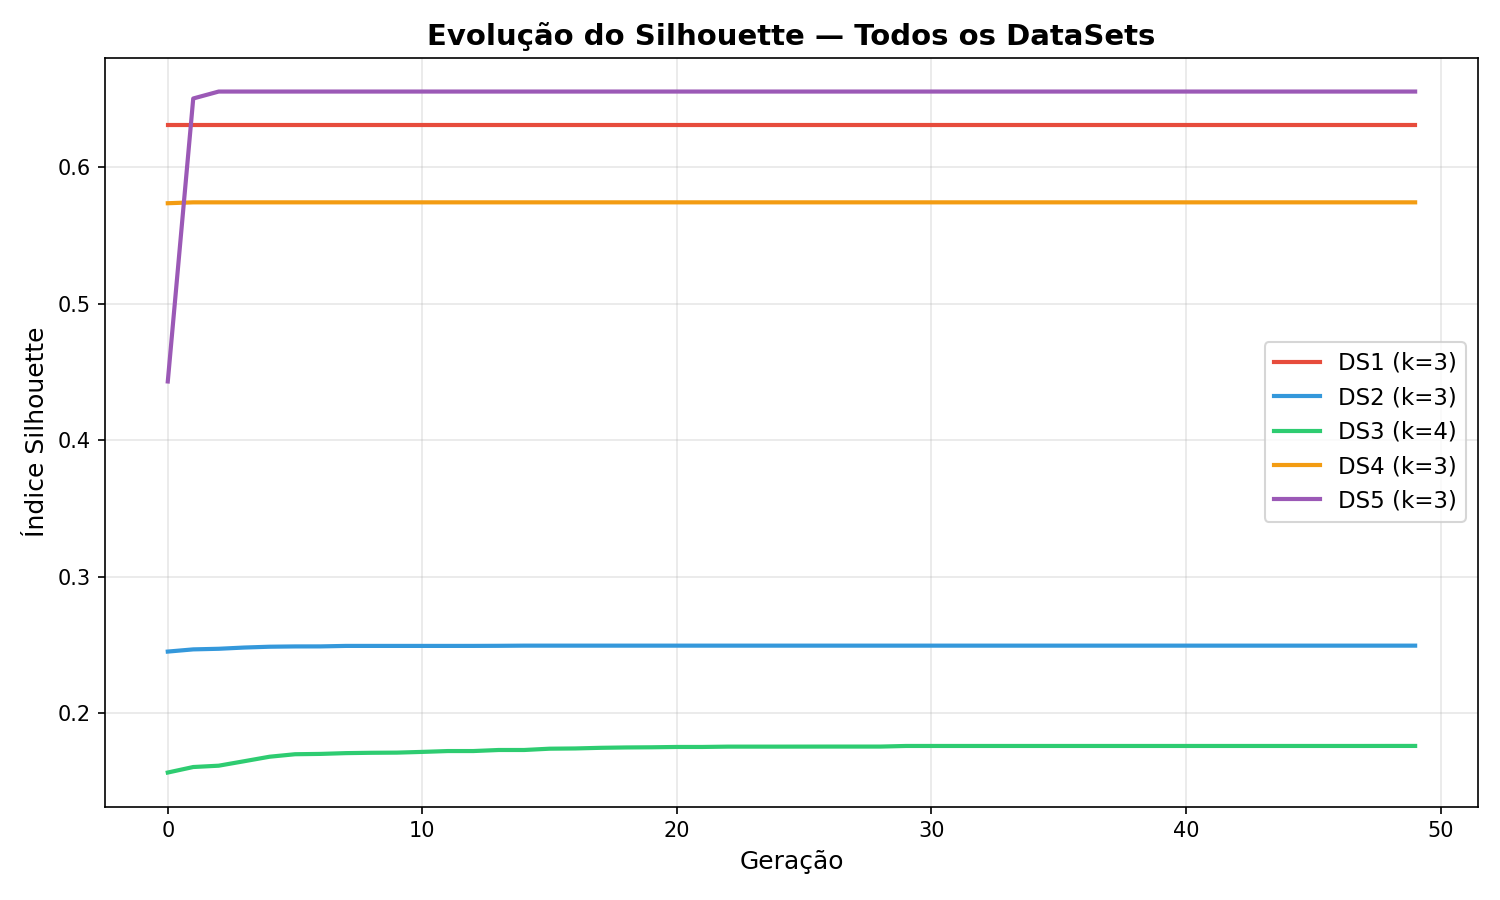
\includegraphics[width=0.85\textwidth]{resultados/etapa3_parametros/evolucao_consolidado.png}
\caption{Evolução consolidada do Silhouette nos cinco datasets.}
\label{fig:evolucao-consolidada}
\end{figure}

\begin{figure}[H]
\centering
\begin{subfigure}{0.48\textwidth}
\centering
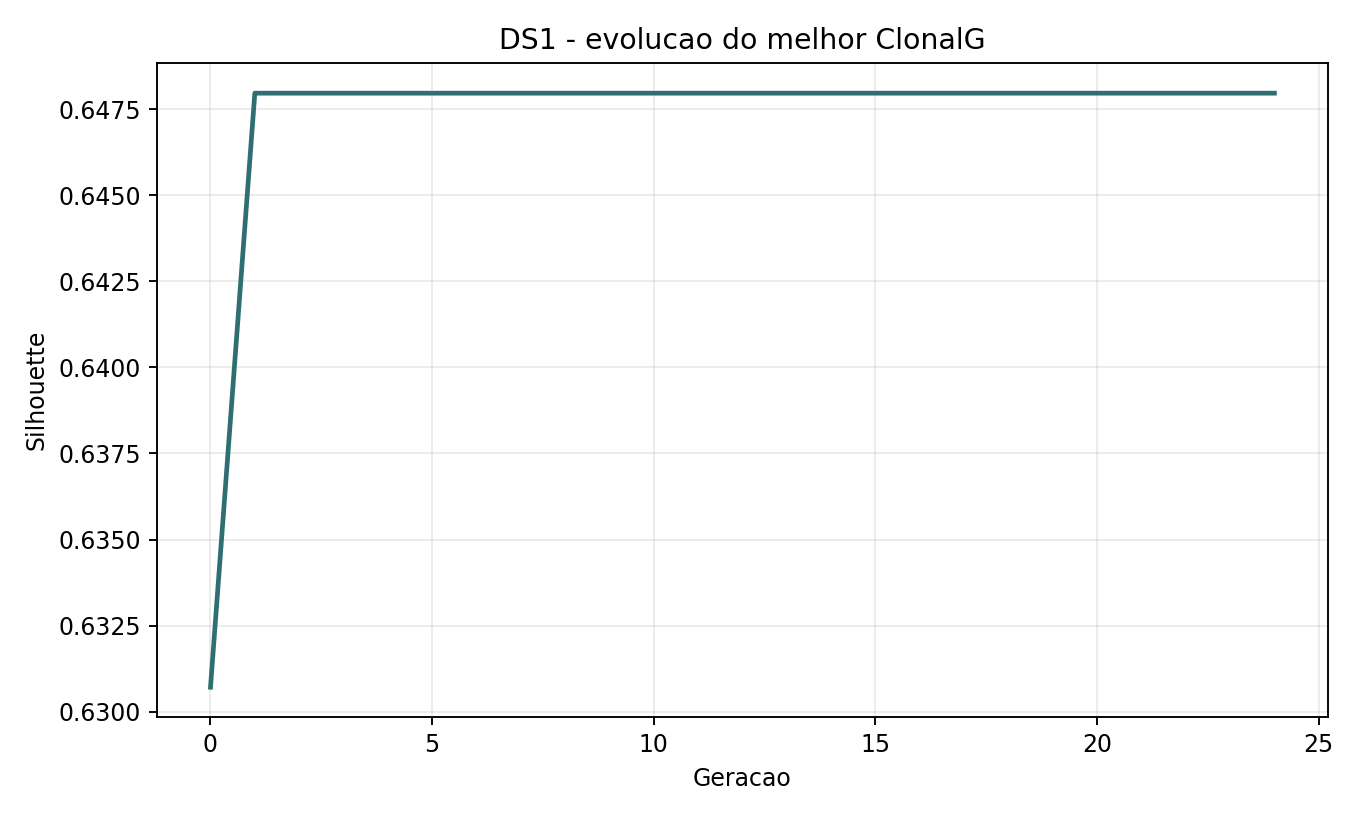
\includegraphics[width=\textwidth]{resultados/comparativo_final/evolucao_clonalg_ds1.png}
\caption{DS1}
\end{subfigure}
\begin{subfigure}{0.48\textwidth}
\centering
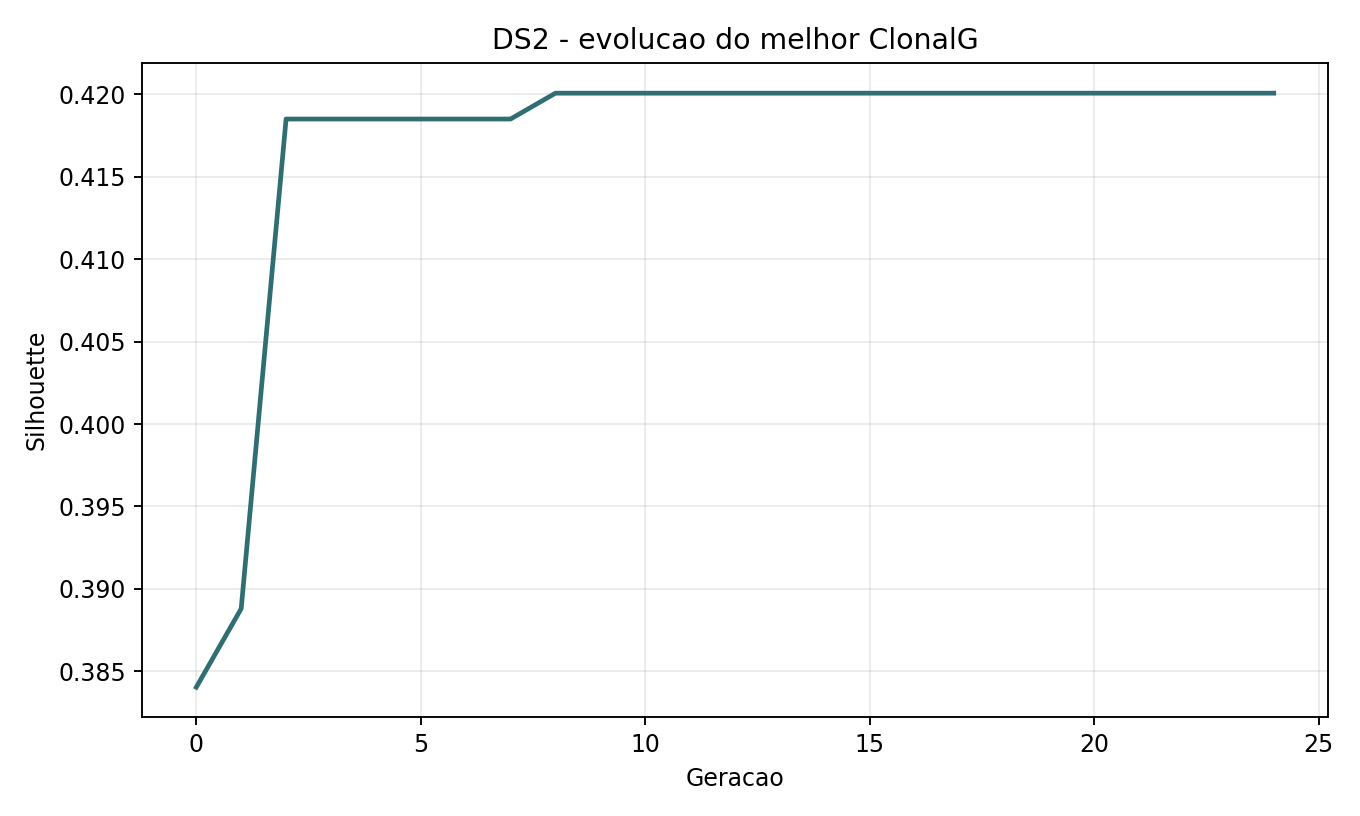
\includegraphics[width=\textwidth]{resultados/comparativo_final/evolucao_clonalg_ds2.png}
\caption{DS2}
\end{subfigure}

\begin{subfigure}{0.48\textwidth}
\centering
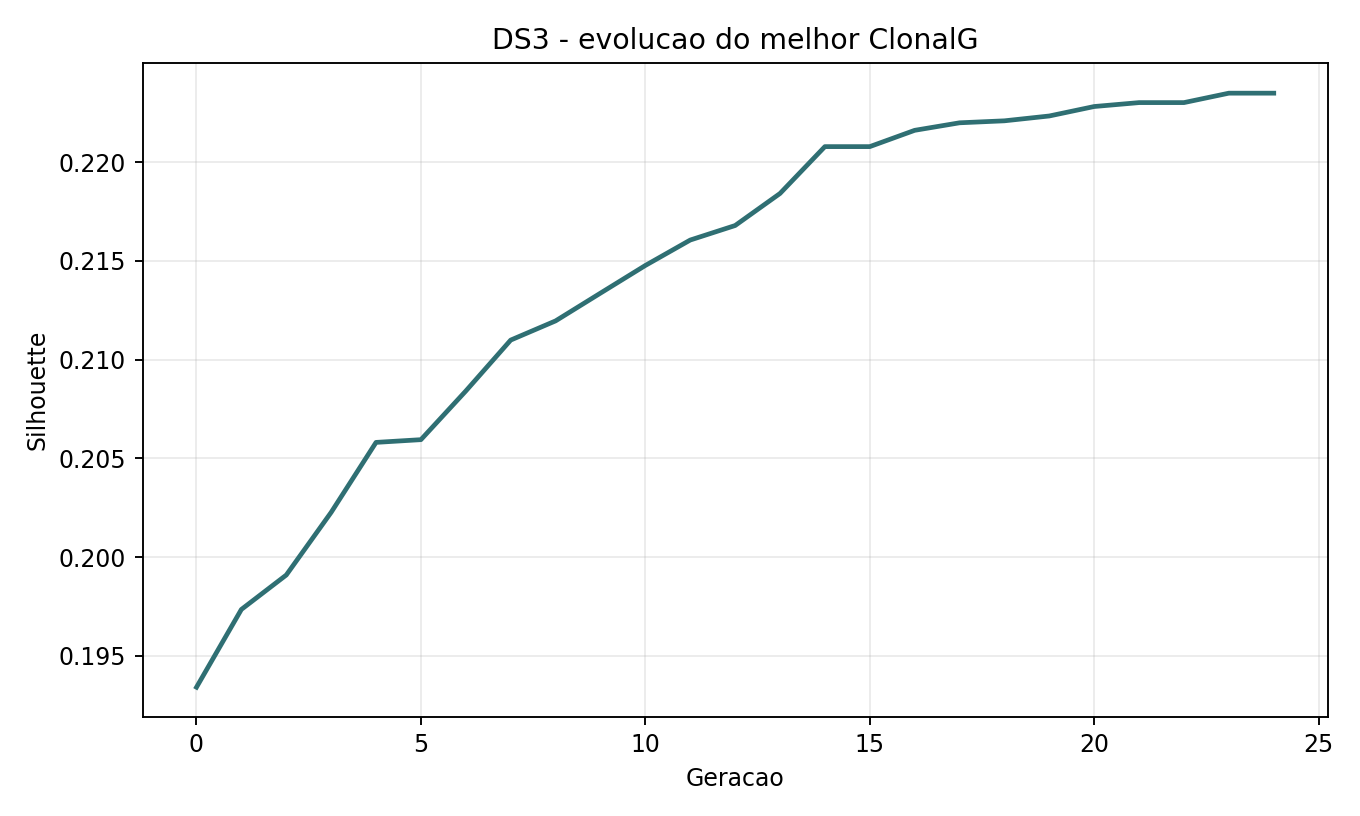
\includegraphics[width=\textwidth]{resultados/comparativo_final/evolucao_clonalg_ds3.png}
\caption{DS3}
\end{subfigure}
\begin{subfigure}{0.48\textwidth}
\centering
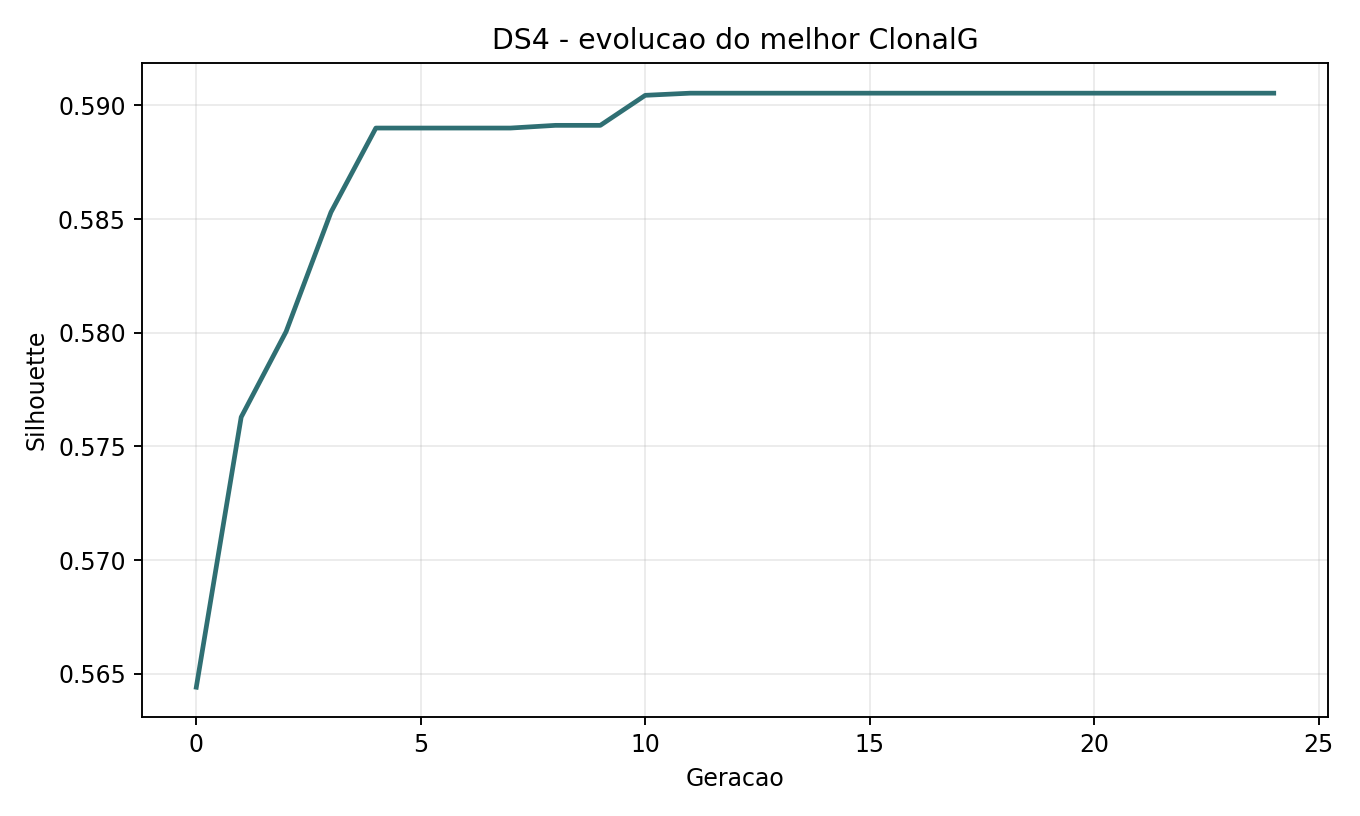
\includegraphics[width=\textwidth]{resultados/comparativo_final/evolucao_clonalg_ds4.png}
\caption{DS4}
\end{subfigure}

\begin{subfigure}{0.55\textwidth}
\centering
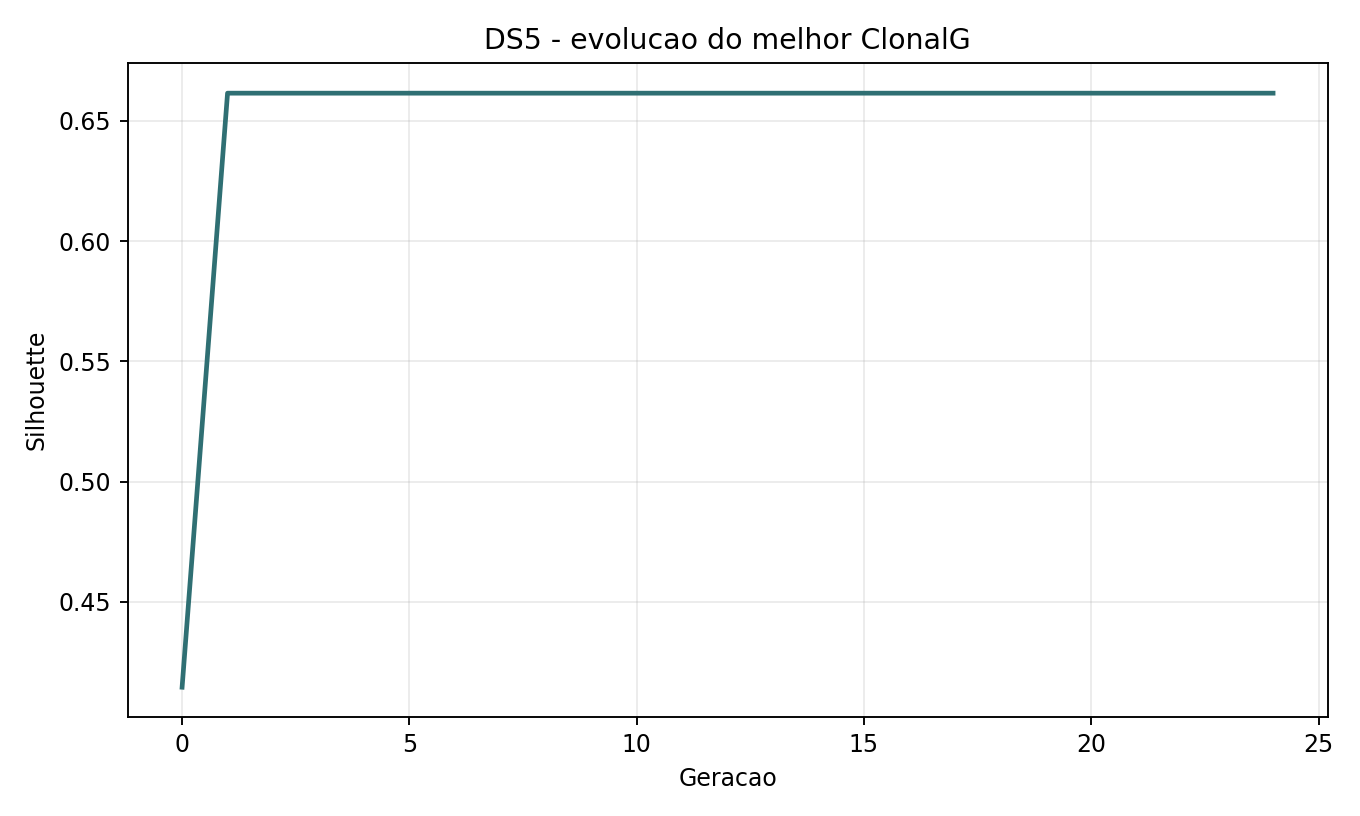
\includegraphics[width=\textwidth]{resultados/comparativo_final/evolucao_clonalg_ds5.png}
\caption{DS5}
\end{subfigure}
\caption{Evolução do melhor ClonalG no comparativo final.}
\label{fig:evolucao-final}
\end{figure}

\subsection{Impacto dos parâmetros}
A Figura~\ref{fig:impacto-parametros} resume o impacto médio dos parâmetros testados sobre o Silhouette. O número de anticorpos altera a capacidade de exploração populacional; o fator \(\rho\) controla a intensidade da busca local; a taxa de substituição regula diversidade; e a taxa de seleção determina quantos candidatos de alta afinidade participam da clonagem.

\begin{figure}[H]
\centering
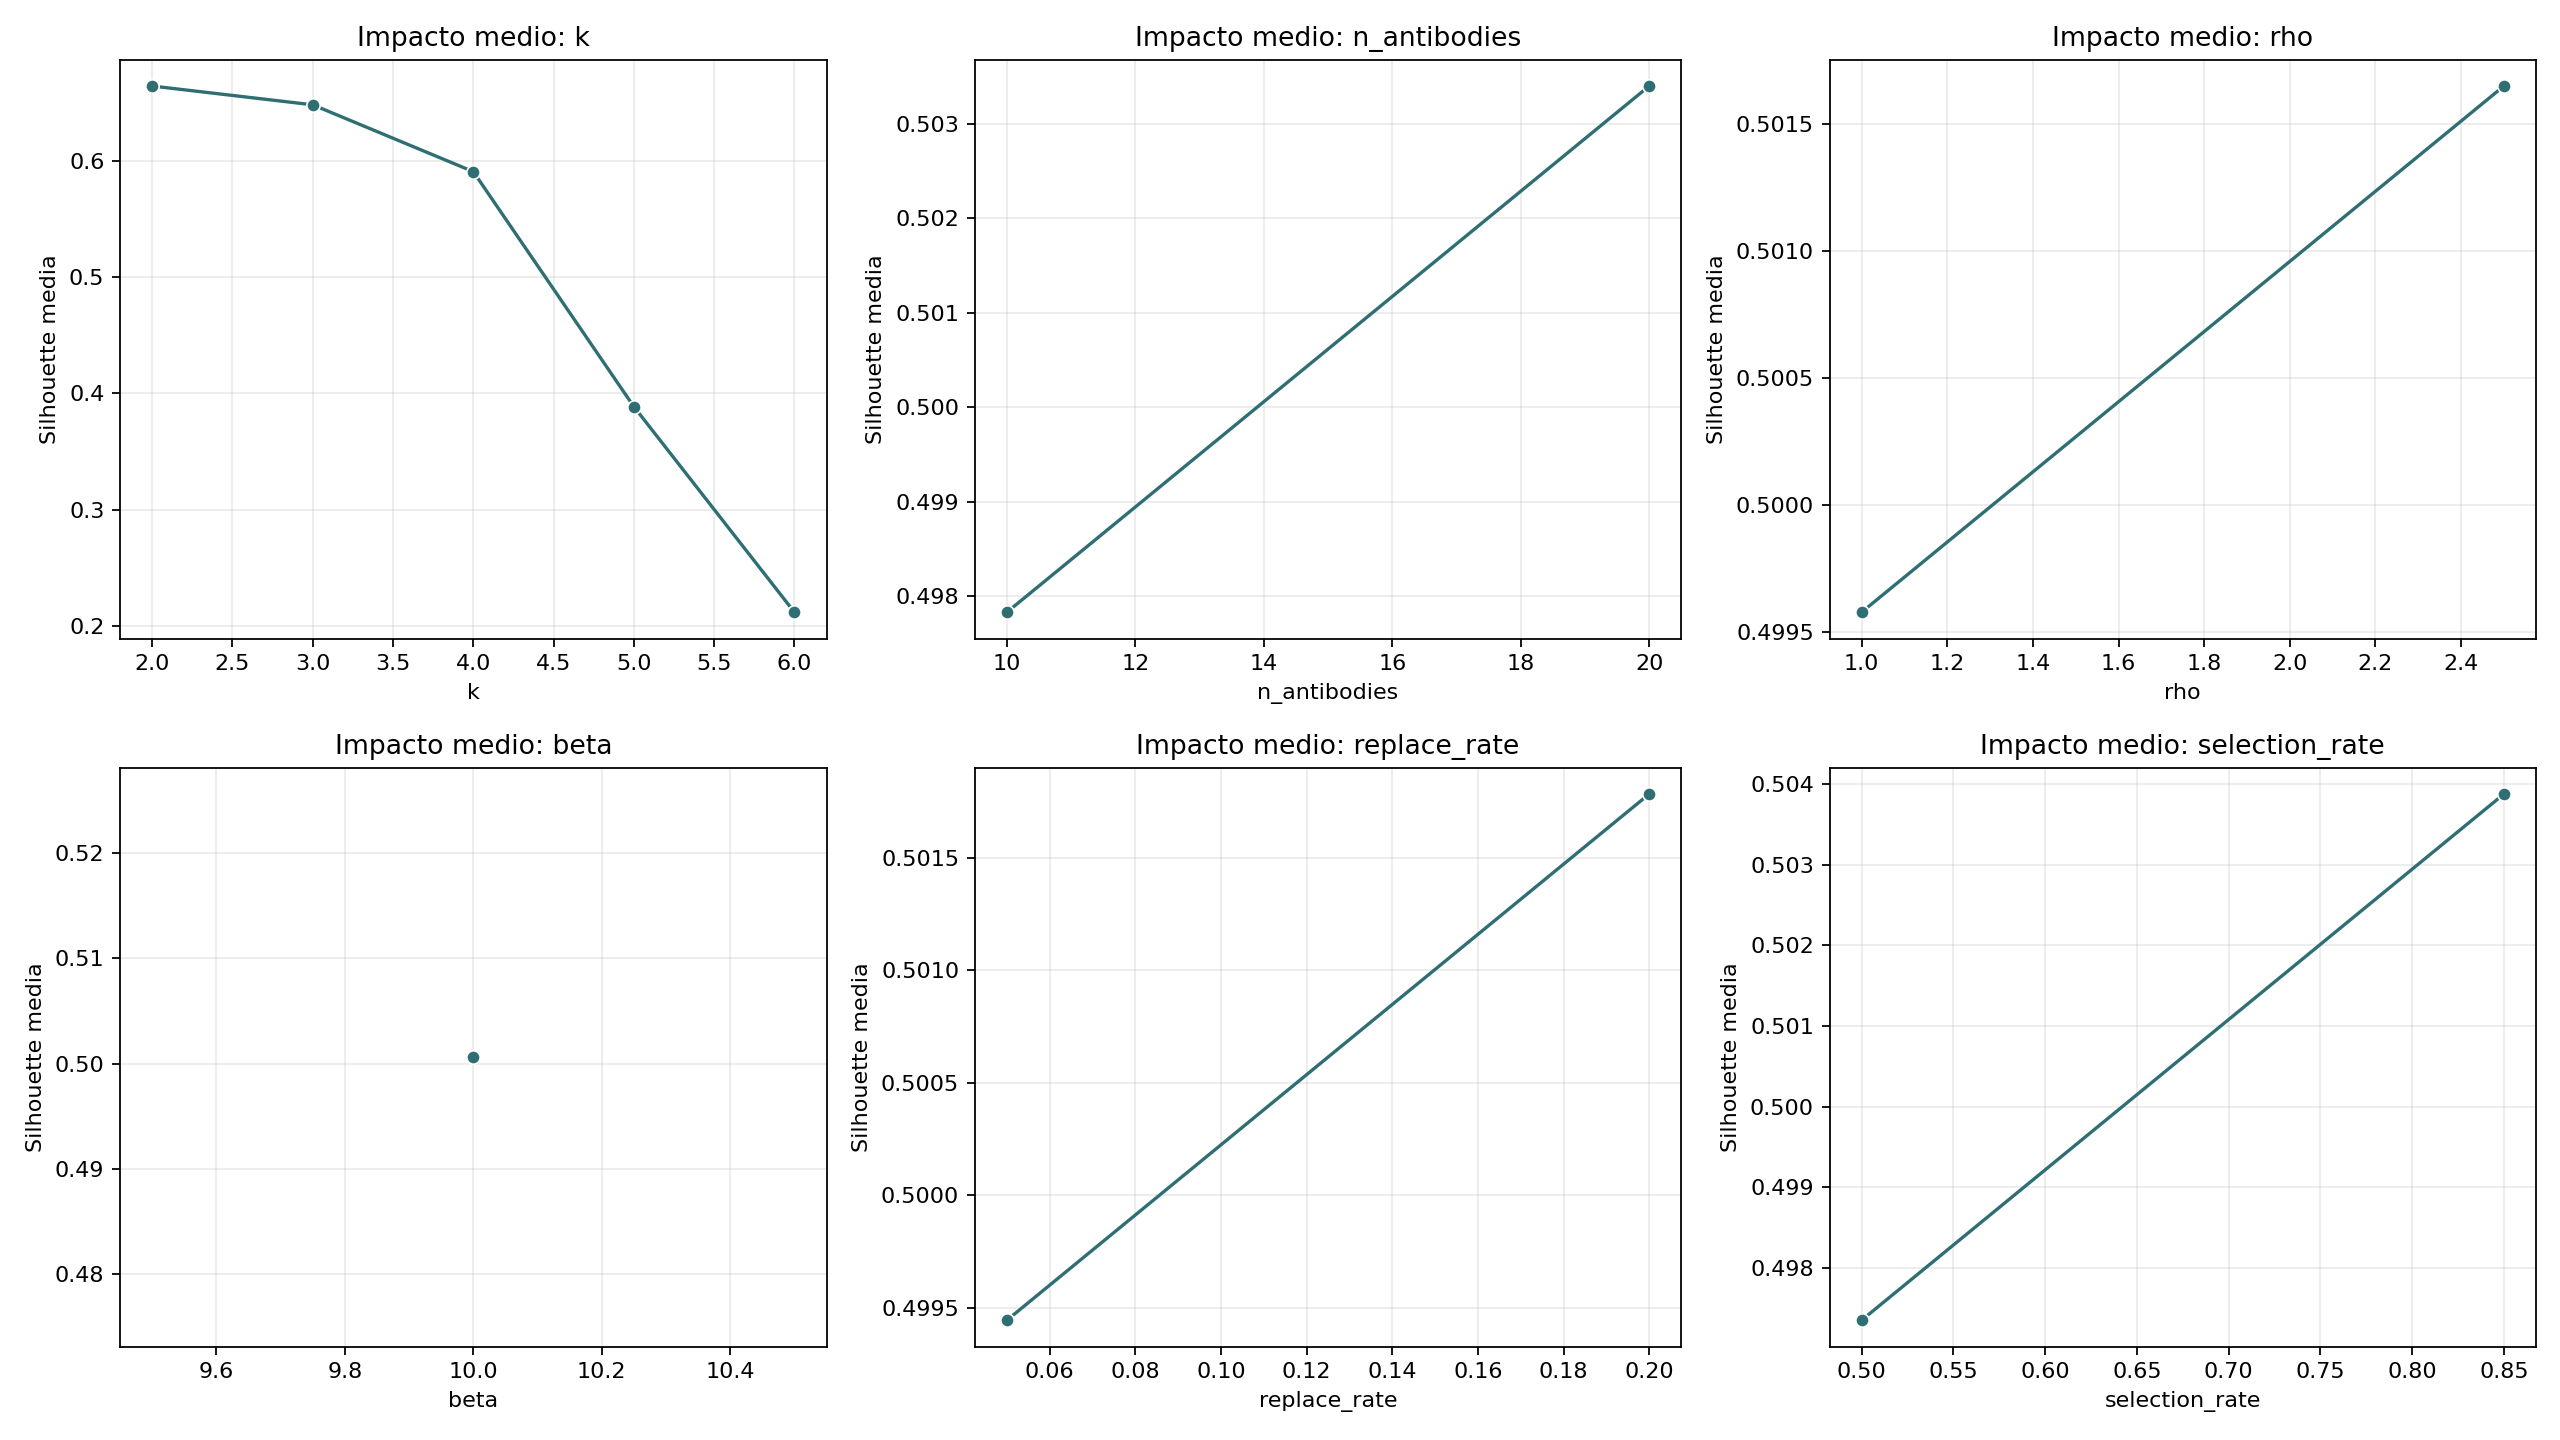
\includegraphics[width=0.95\textwidth]{resultados/etapa3_parametros/impacto_parametros_grid.png}
\caption{Impacto médio dos parâmetros avaliados na busca em grade.}
\label{fig:impacto-parametros}
\end{figure}

\begin{figure}[H]
\centering
\begin{subfigure}{0.48\textwidth}
\centering
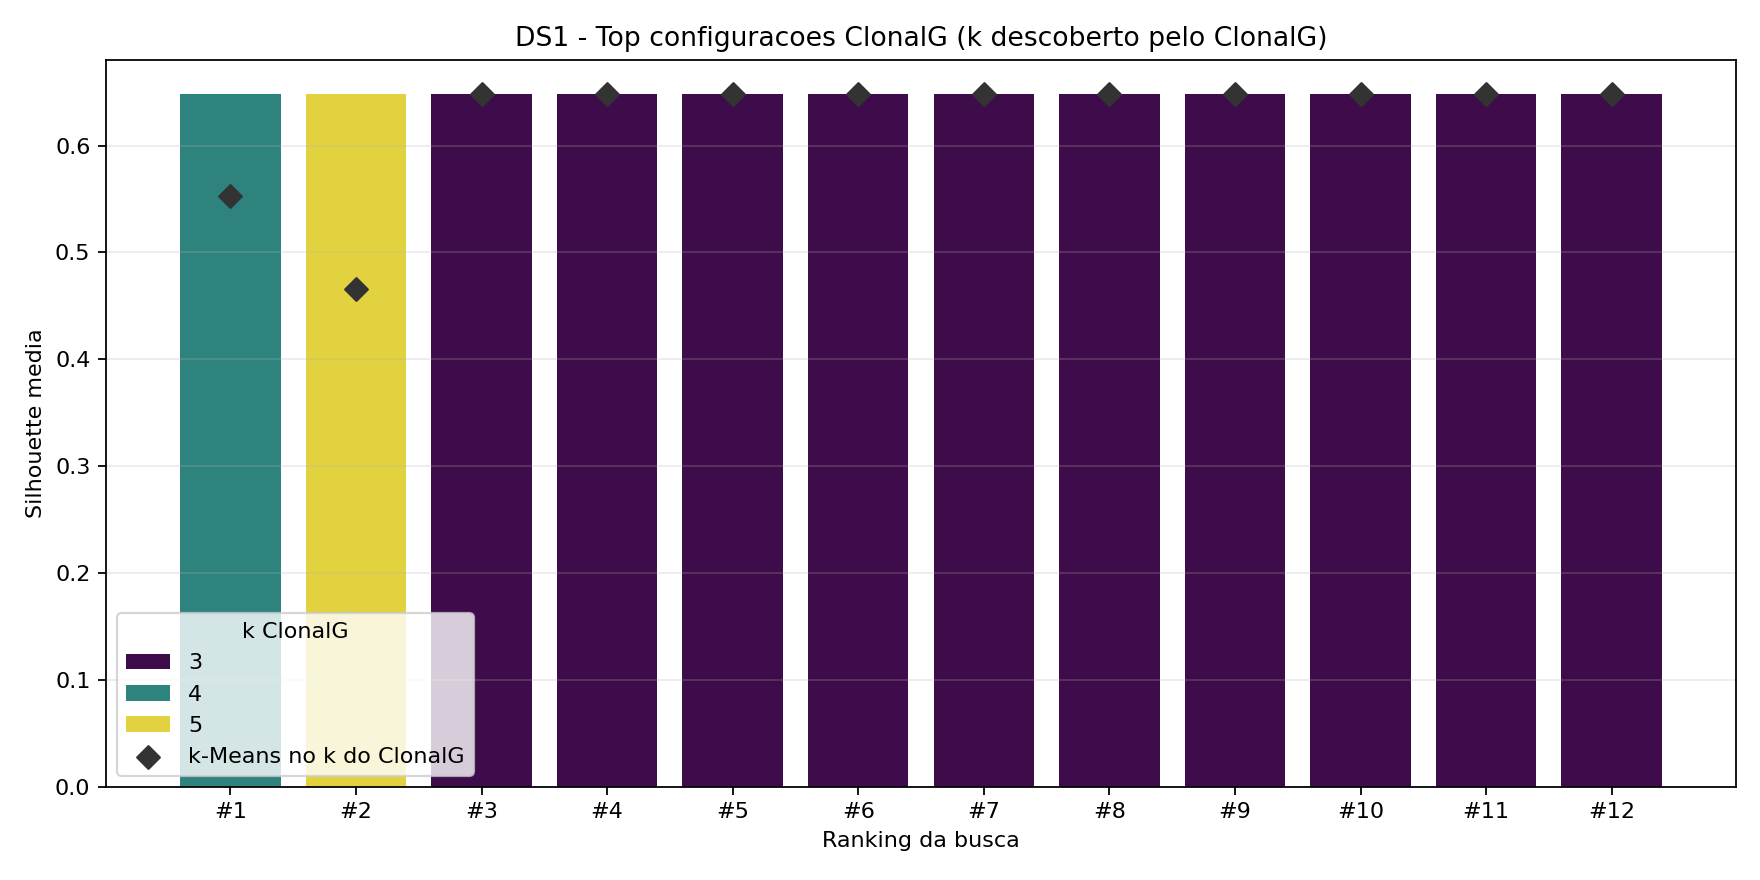
\includegraphics[width=\textwidth]{resultados/etapa3_parametros/ranking_ds1.png}
\caption{DS1}
\end{subfigure}
\begin{subfigure}{0.48\textwidth}
\centering
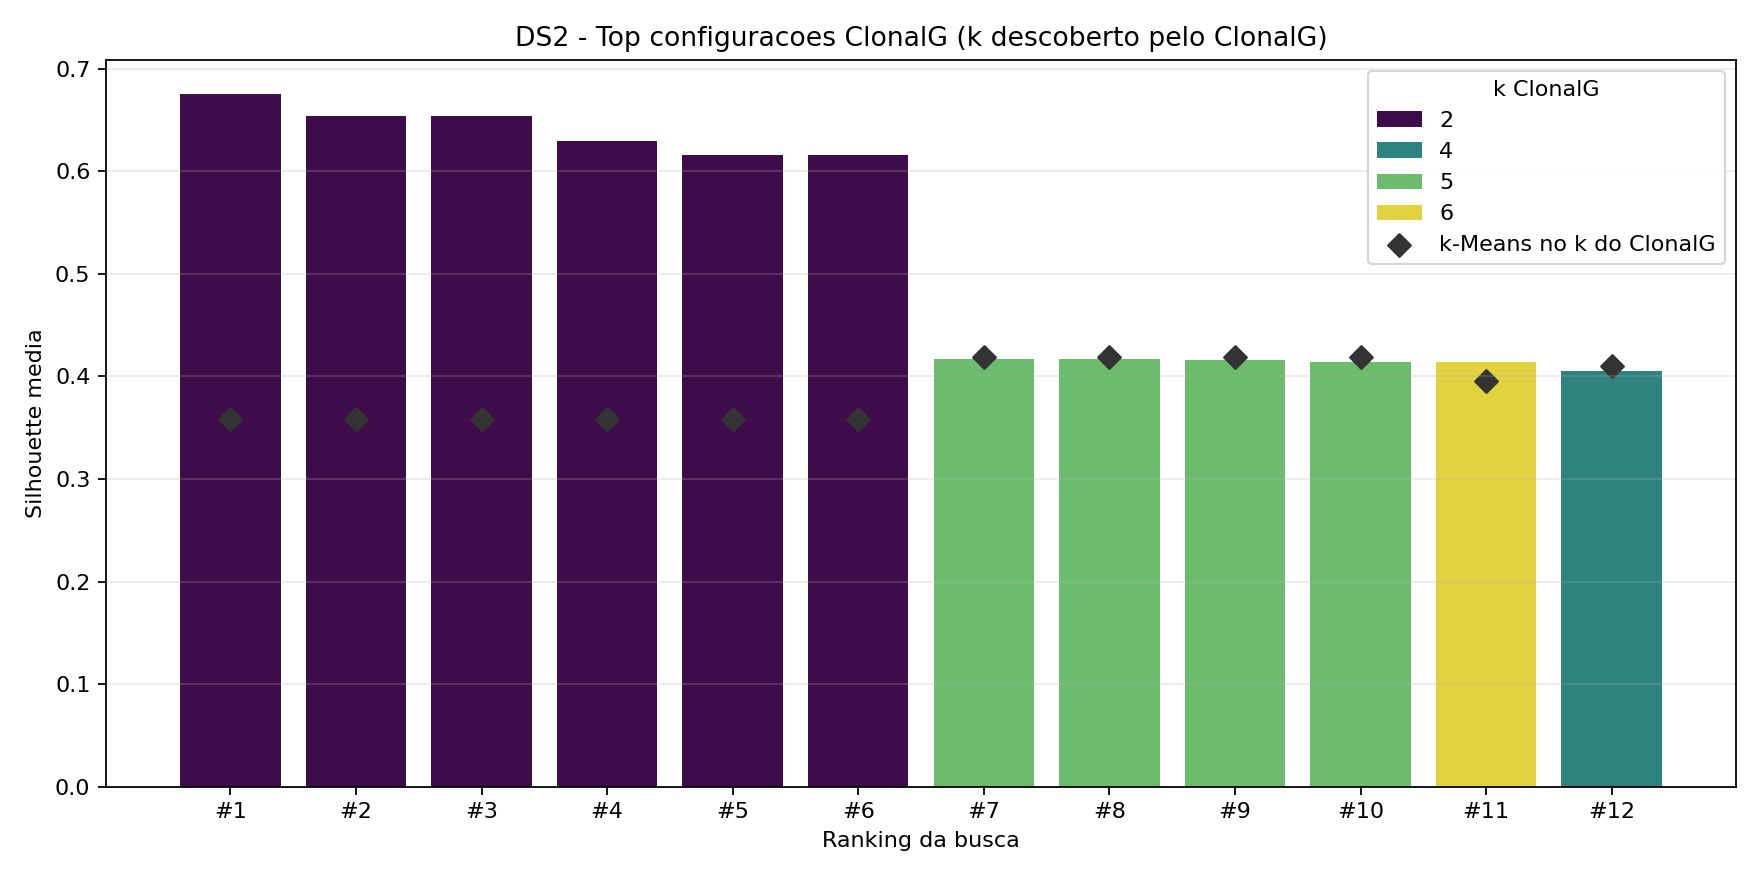
\includegraphics[width=\textwidth]{resultados/etapa3_parametros/ranking_ds2.png}
\caption{DS2}
\end{subfigure}

\begin{subfigure}{0.48\textwidth}
\centering
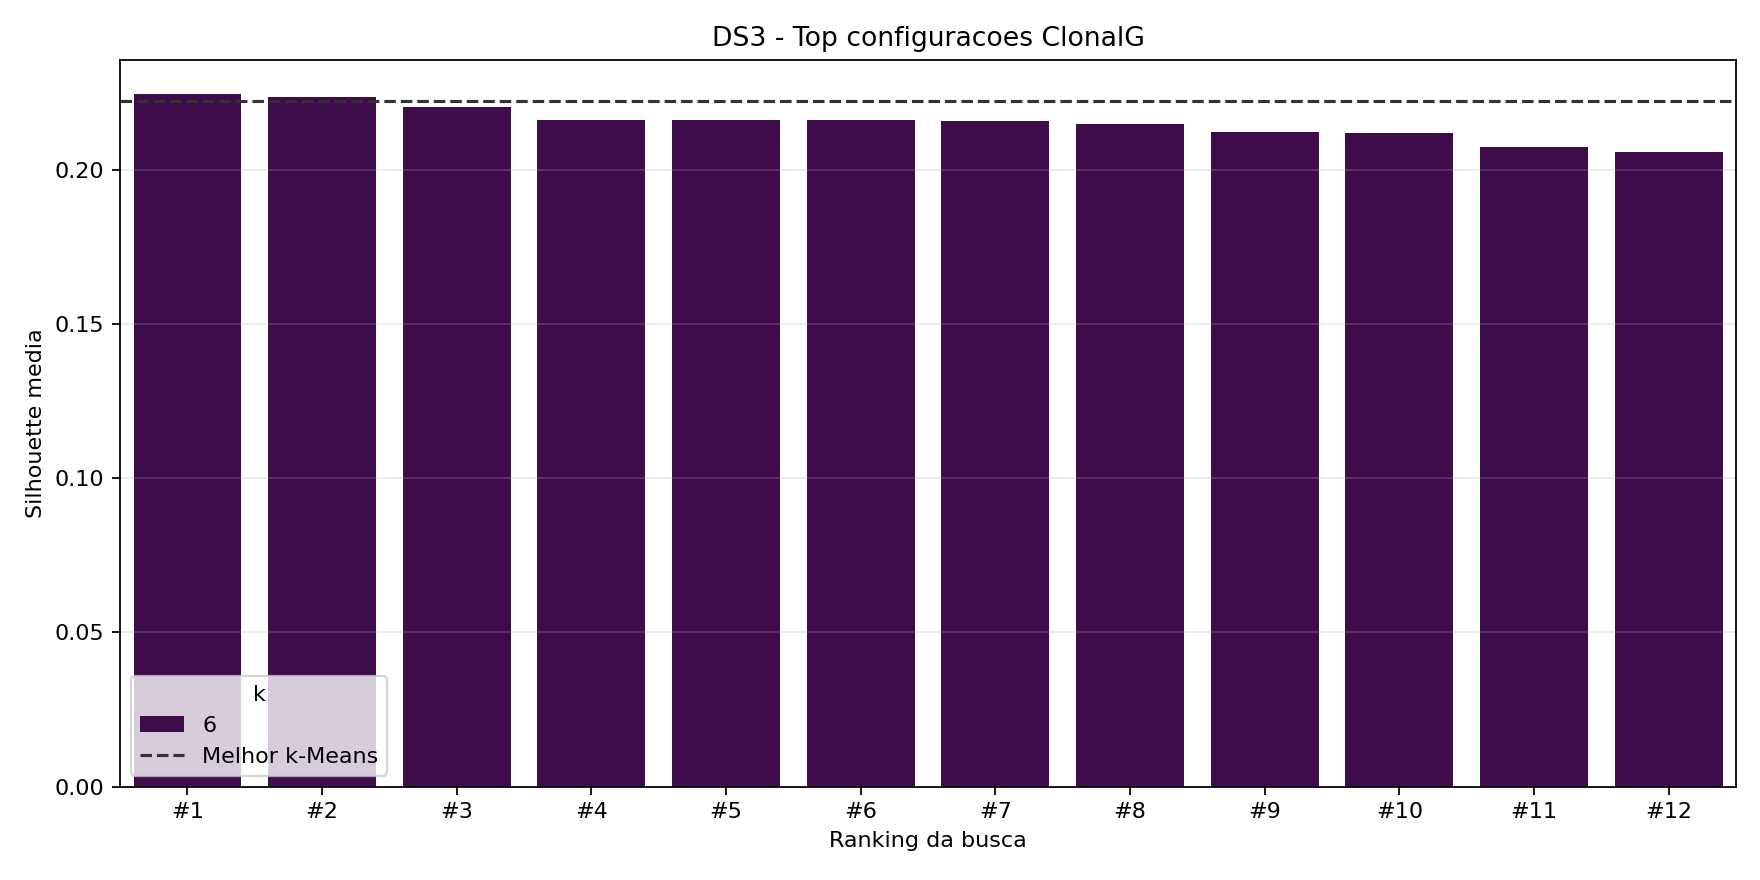
\includegraphics[width=\textwidth]{resultados/etapa3_parametros/ranking_ds3.png}
\caption{DS3}
\end{subfigure}
\begin{subfigure}{0.48\textwidth}
\centering
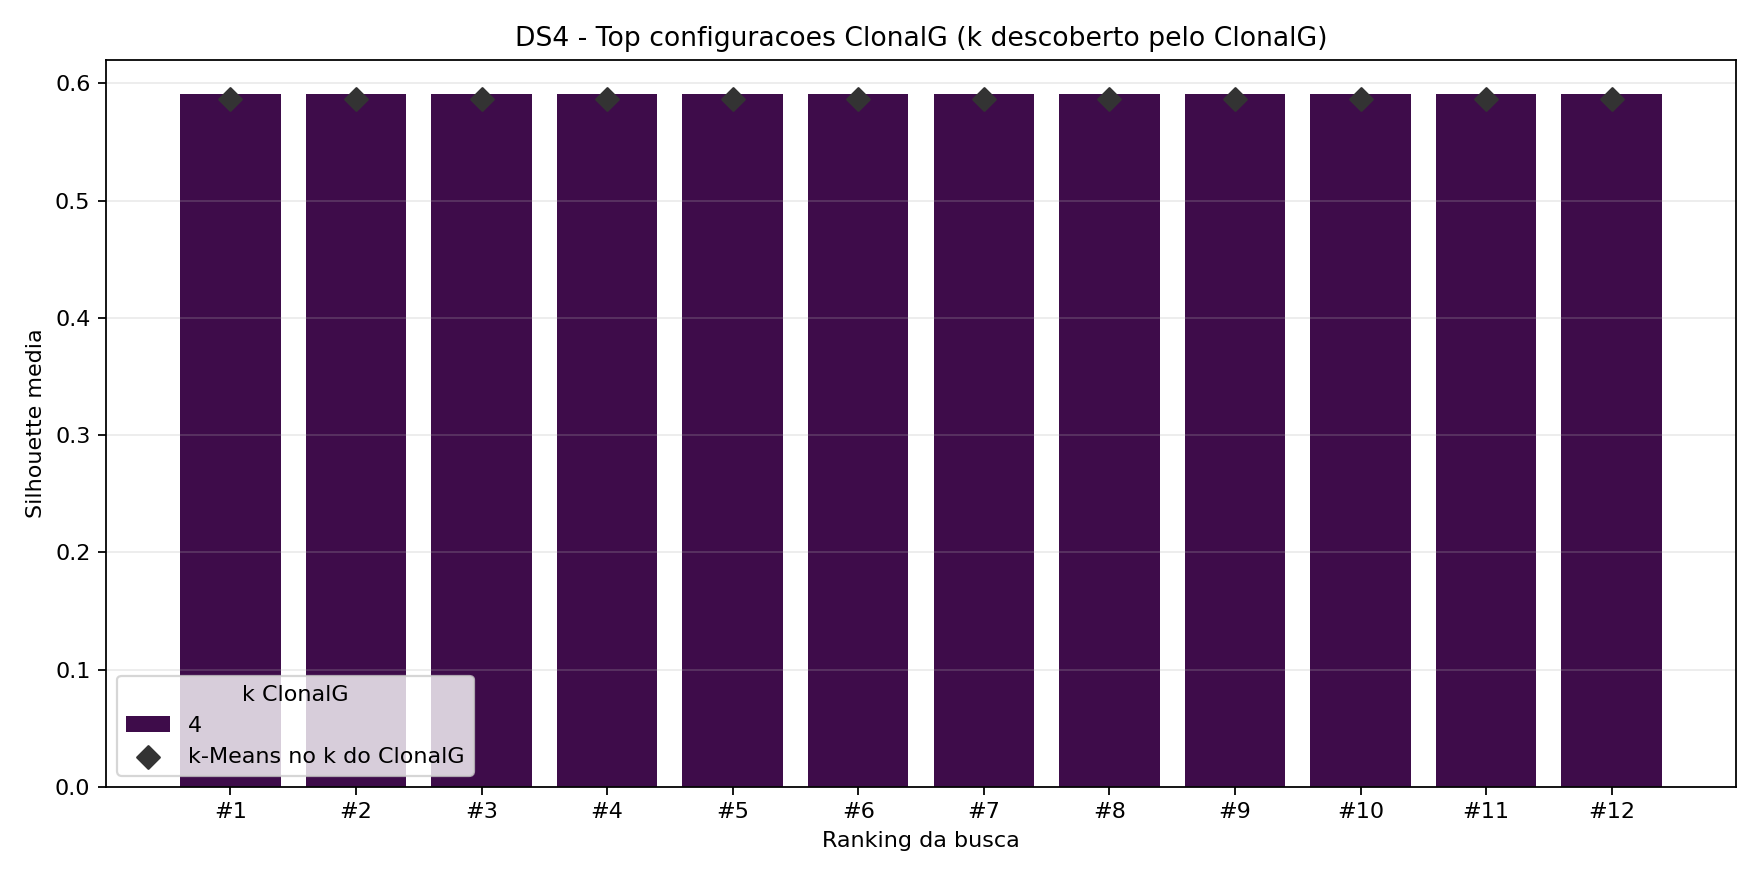
\includegraphics[width=\textwidth]{resultados/etapa3_parametros/ranking_ds4.png}
\caption{DS4}
\end{subfigure}

\begin{subfigure}{0.55\textwidth}
\centering
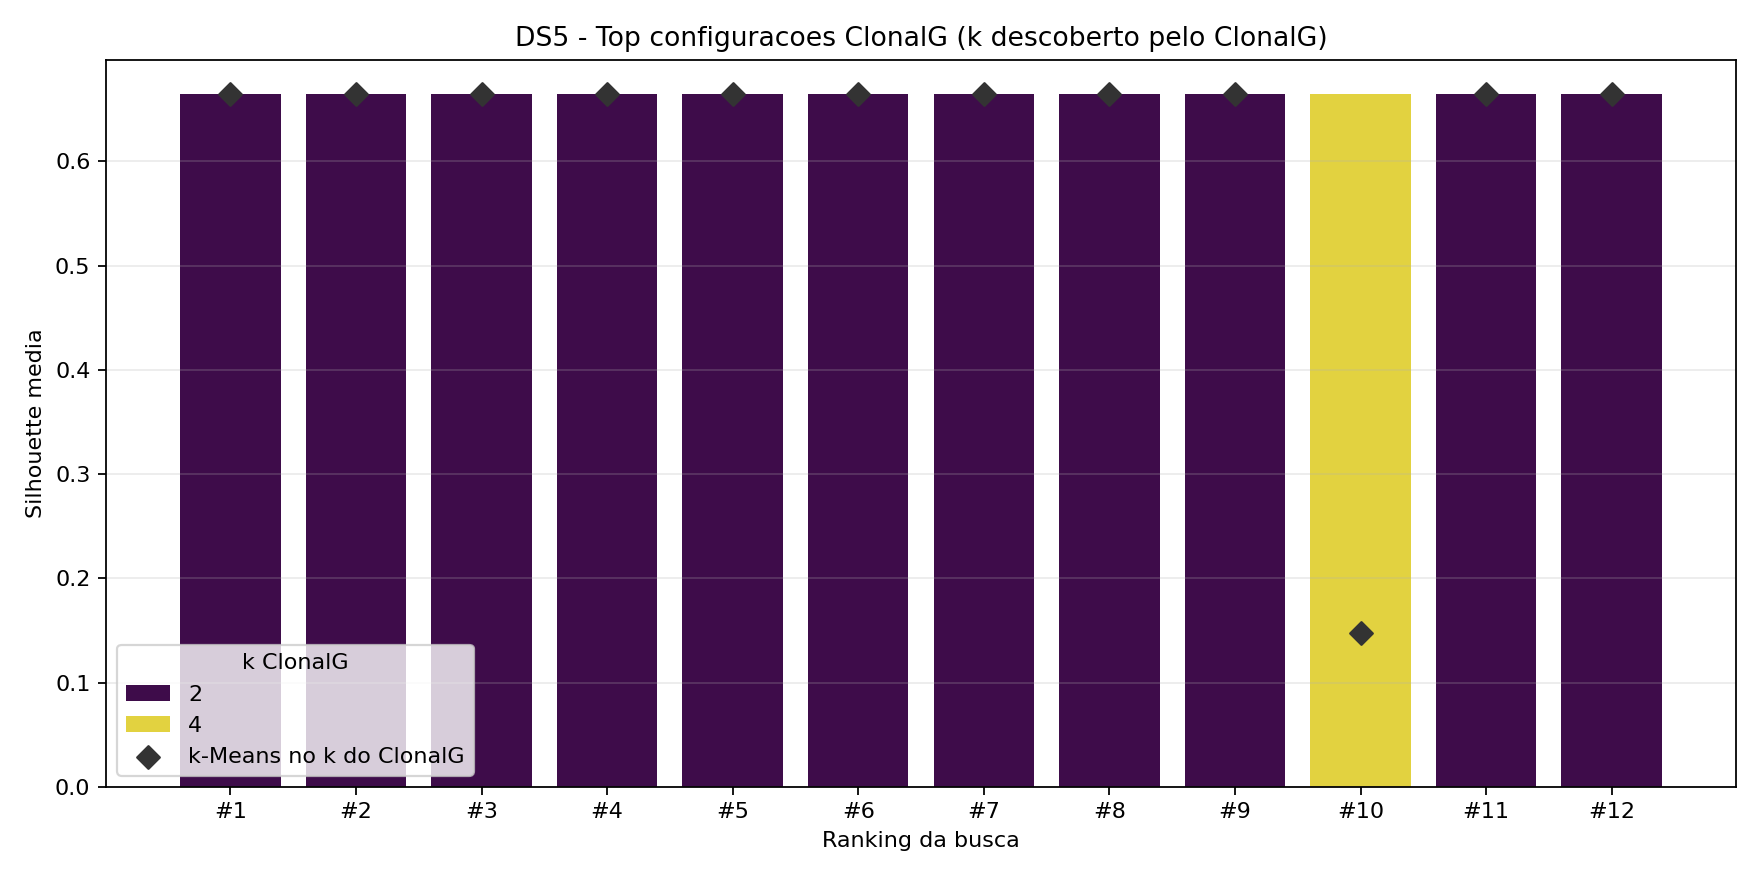
\includegraphics[width=\textwidth]{resultados/etapa3_parametros/ranking_ds5.png}
\caption{DS5}
\end{subfigure}
\caption{Ranking das melhores configurações do ClonalG por dataset durante a busca.}
\label{fig:rankings}
\end{figure}

\subsection{Visualização dos agrupamentos}
As Figuras~\ref{fig:comparacao-ds1-ds2}, \ref{fig:comparacao-ds3-ds4} e \ref{fig:comparacao-ds5} mostram os agrupamentos gerados pelo ClonalG e pelo k-Means. Nos datasets multidimensionais, os pontos e centroides foram projetados por PCA para visualização. As métricas, entretanto, foram calculadas no espaço padronizado completo.

\begin{figure}[H]
\centering
\begin{subfigure}{0.49\textwidth}
\centering
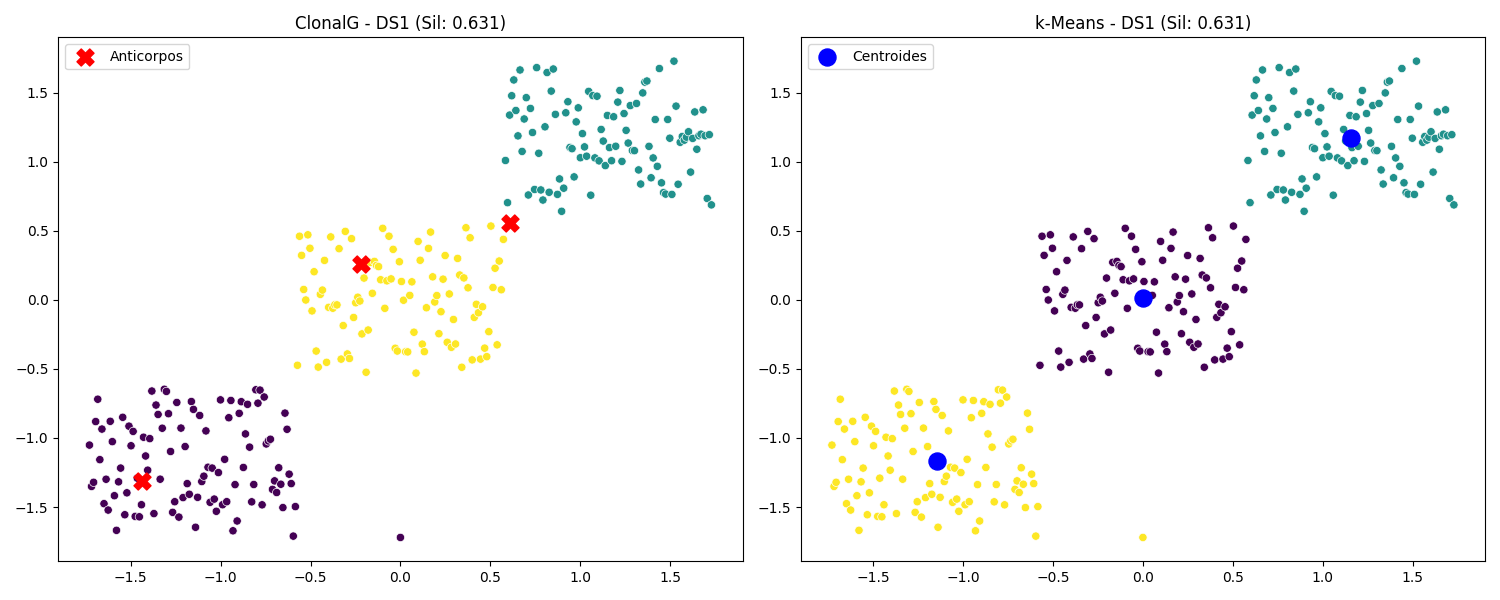
\includegraphics[width=\textwidth]{resultados/comparativo_final/comparacao_ds1.png}
\caption{DataSet 1}
\end{subfigure}
\begin{subfigure}{0.49\textwidth}
\centering
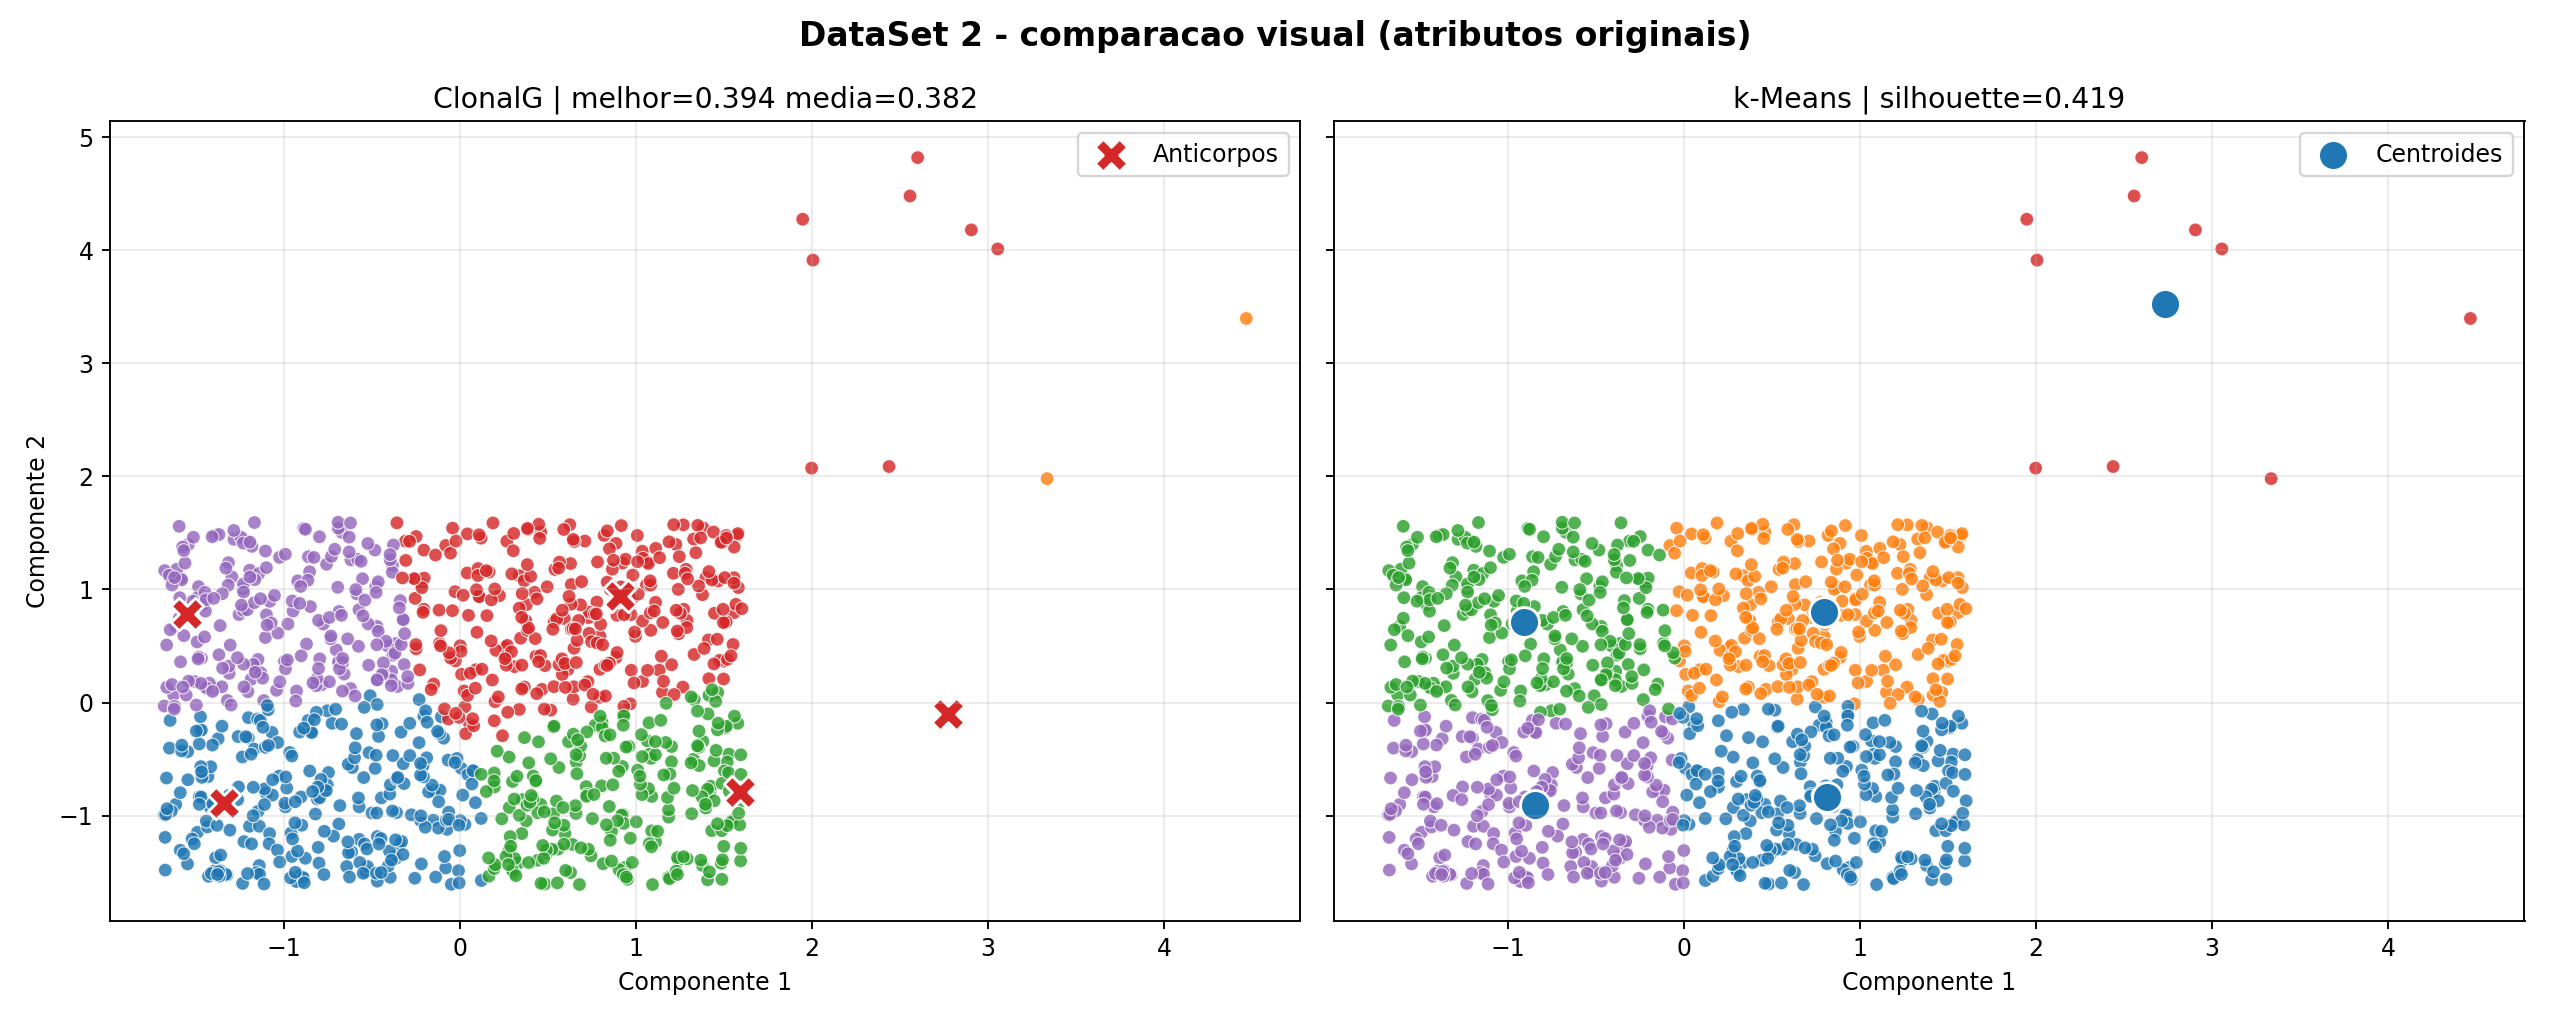
\includegraphics[width=\textwidth]{resultados/comparativo_final/comparacao_ds2.png}
\caption{DataSet 2}
\end{subfigure}
\caption{Comparação visual entre ClonalG e k-Means nos DataSets 1 e 2.}
\label{fig:comparacao-ds1-ds2}
\end{figure}

\begin{figure}[H]
\centering
\begin{subfigure}{0.49\textwidth}
\centering
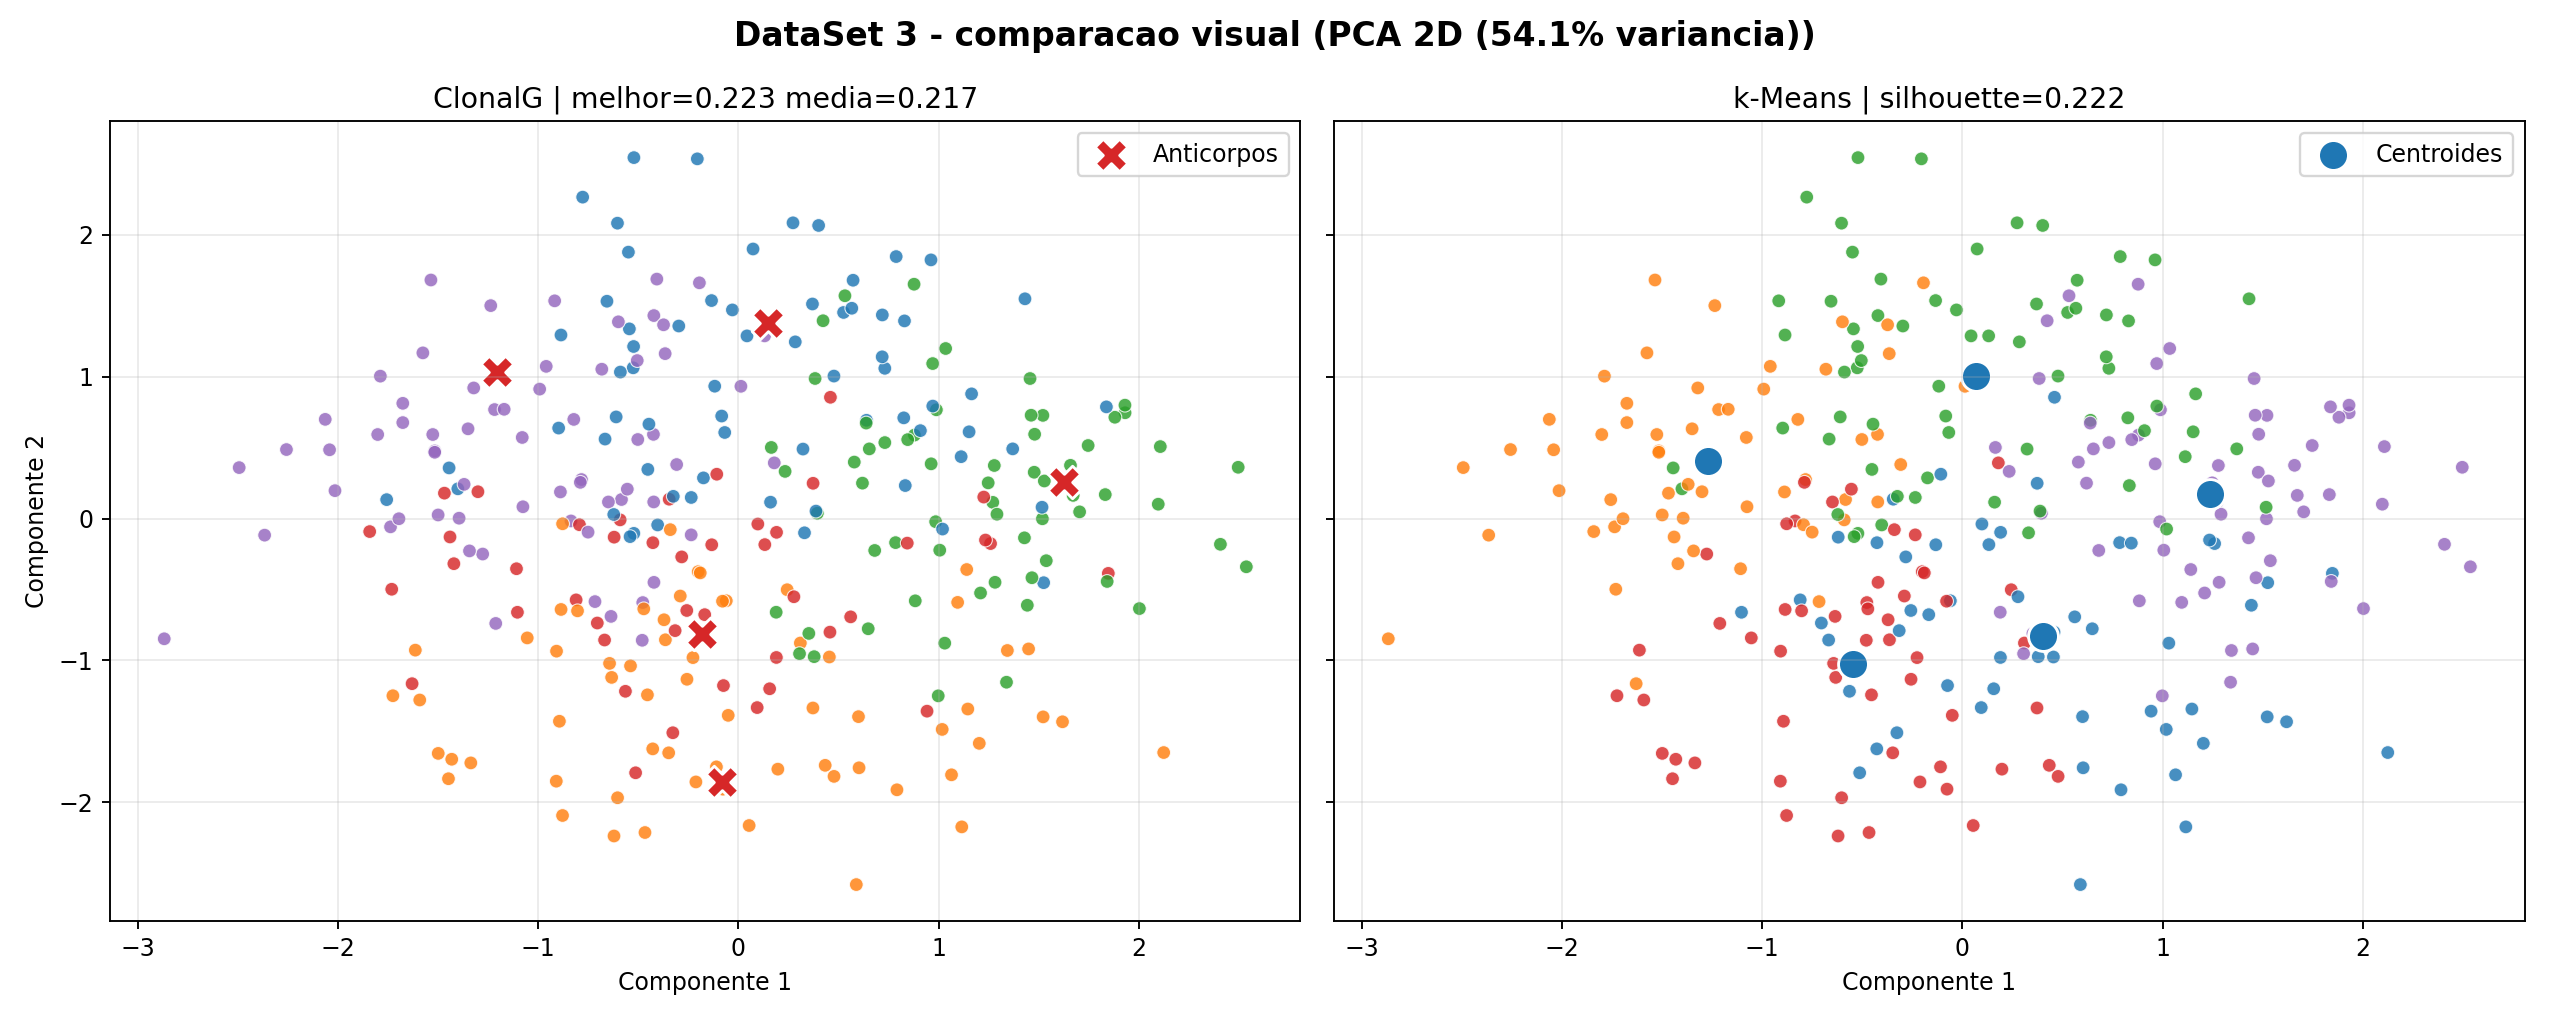
\includegraphics[width=\textwidth]{resultados/comparativo_final/comparacao_ds3.png}
\caption{DataSet 3}
\end{subfigure}
\begin{subfigure}{0.49\textwidth}
\centering
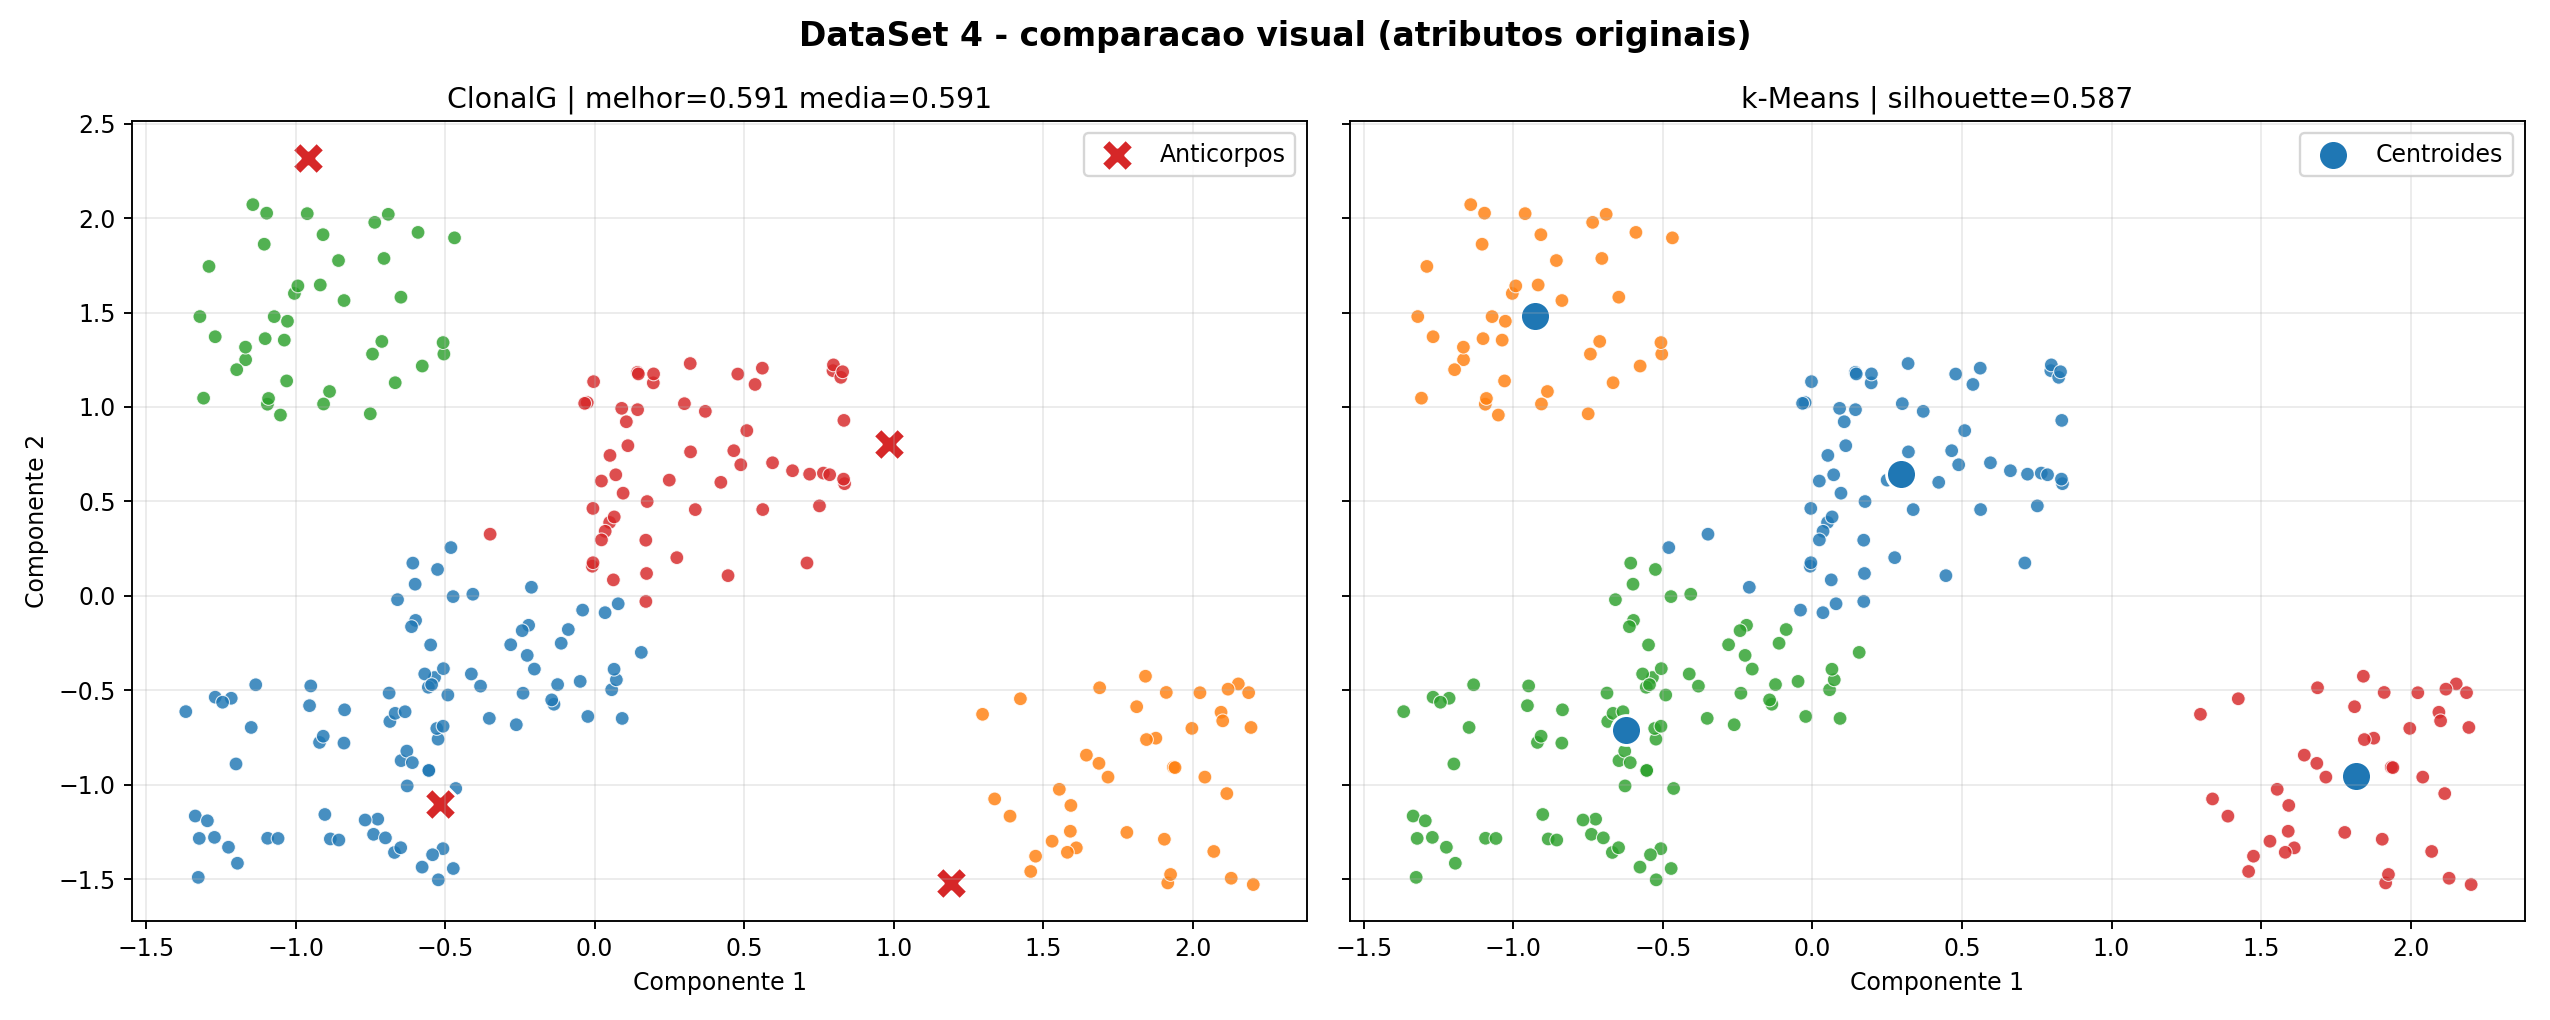
\includegraphics[width=\textwidth]{resultados/comparativo_final/comparacao_ds4.png}
\caption{DataSet 4}
\end{subfigure}
\caption{Comparação visual entre ClonalG e k-Means nos DataSets 3 e 4.}
\label{fig:comparacao-ds3-ds4}
\end{figure}

\begin{figure}[H]
\centering
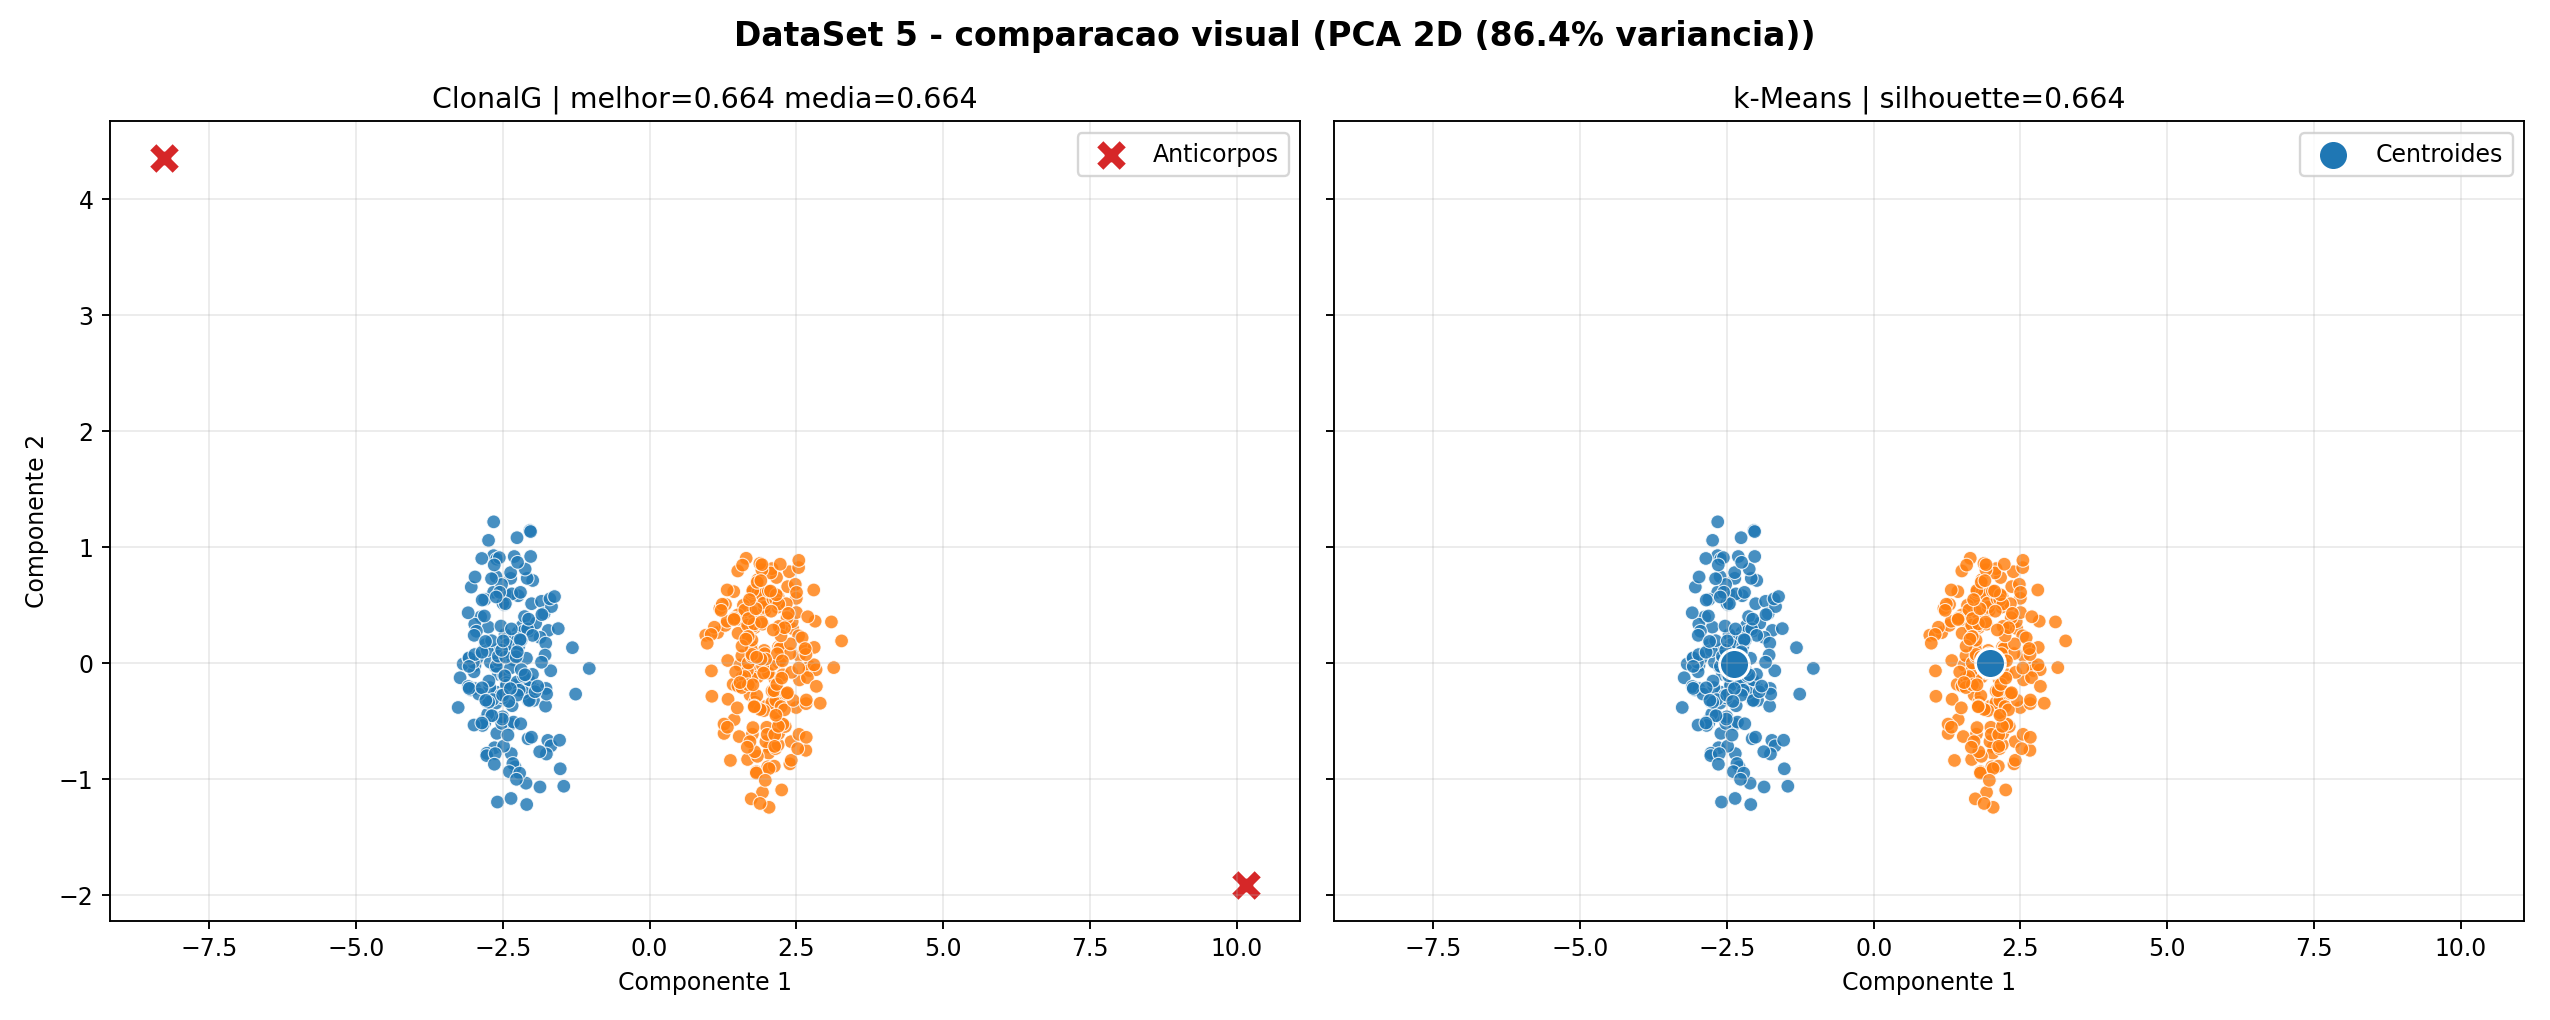
\includegraphics[width=0.85\textwidth]{resultados/comparativo_final/comparacao_ds5.png}
\caption{Comparação visual entre ClonalG e k-Means no DataSet 5.}
\label{fig:comparacao-ds5}
\end{figure}

\subsection{Visualização da descoberta de k}
A Figura~\ref{fig:k-auto-visual} apresenta os agrupamentos obtidos durante a etapa de descoberta automática de \(k\). Esses gráficos ajudam a observar se o número de centroides escolhido pelo ClonalG produz uma partição visualmente plausível.

\begin{figure}[H]
\centering
\begin{subfigure}{0.48\textwidth}
\centering
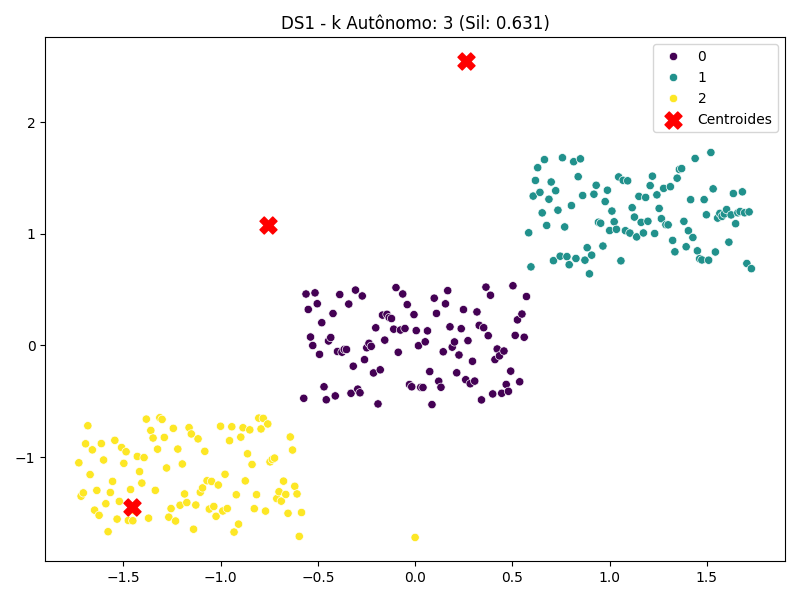
\includegraphics[width=\textwidth]{resultados/etapa4_descoberta_k/descoberta_ds1.png}
\caption{DS1}
\end{subfigure}
\begin{subfigure}{0.48\textwidth}
\centering
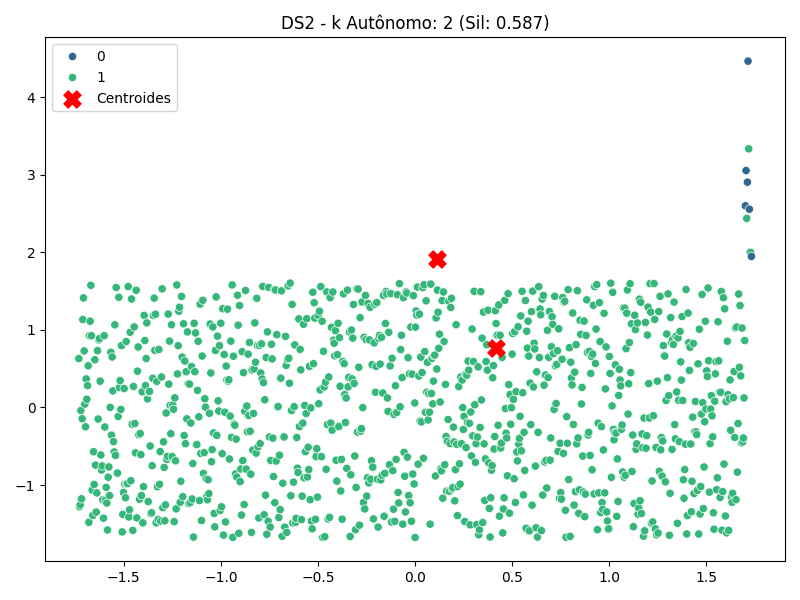
\includegraphics[width=\textwidth]{resultados/etapa4_descoberta_k/descoberta_ds2.png}
\caption{DS2}
\end{subfigure}

\begin{subfigure}{0.48\textwidth}
\centering
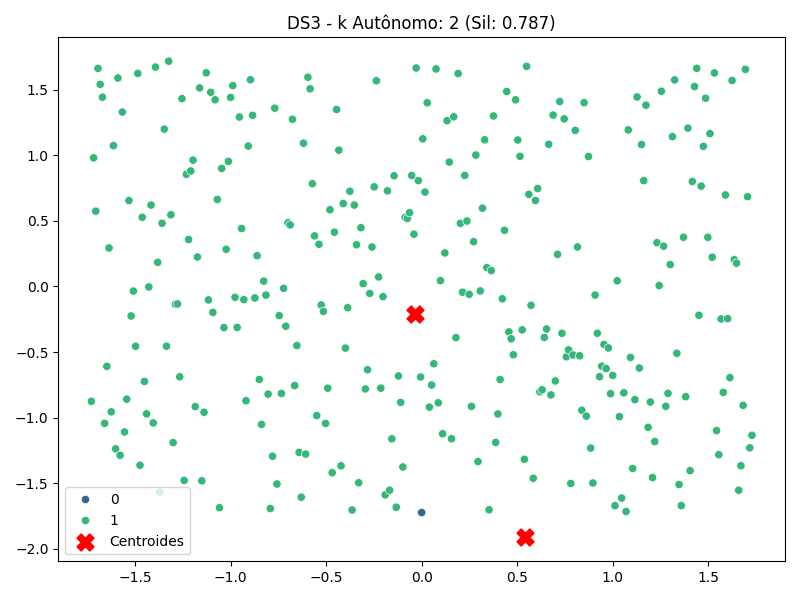
\includegraphics[width=\textwidth]{resultados/etapa4_descoberta_k/descoberta_ds3.png}
\caption{DS3}
\end{subfigure}
\begin{subfigure}{0.48\textwidth}
\centering
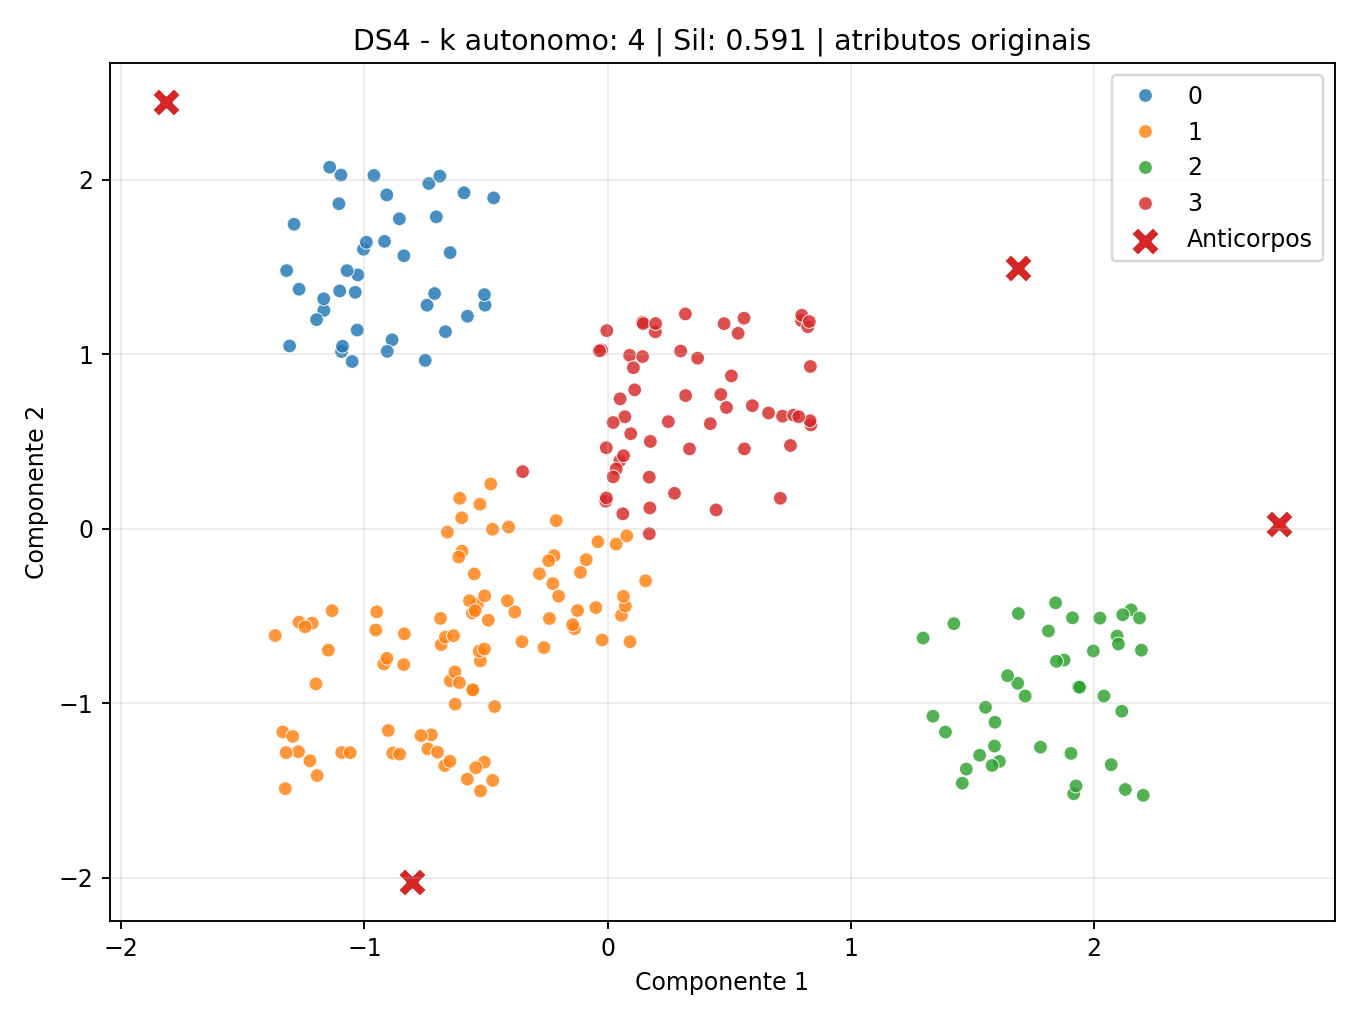
\includegraphics[width=\textwidth]{resultados/etapa4_descoberta_k/descoberta_ds4.png}
\caption{DS4}
\end{subfigure}

\begin{subfigure}{0.55\textwidth}
\centering
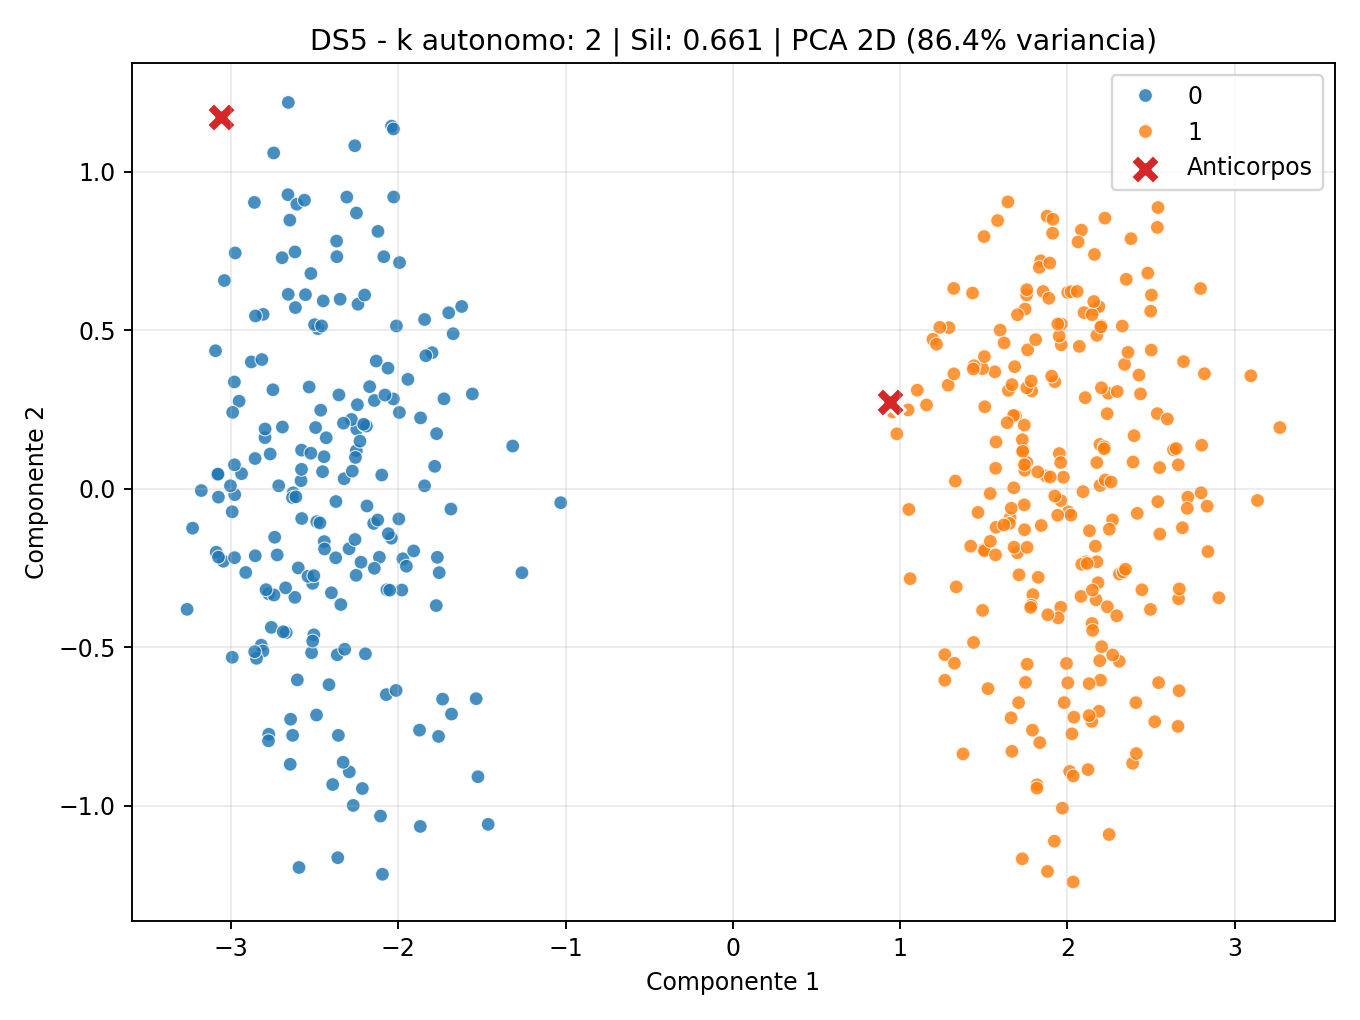
\includegraphics[width=\textwidth]{resultados/etapa4_descoberta_k/descoberta_ds5.png}
\caption{DS5}
\end{subfigure}
\caption{Agrupamentos obtidos pelo ClonalG com descoberta automática de \(k\).}
\label{fig:k-auto-visual}
\end{figure}

\section{Discussão}

\subsection{Comparação técnica com k-Means}
O ClonalG apresentou desempenho competitivo em relação ao k-Means. Nos DataSets 1 e 5, os dois métodos obtiveram essencialmente o mesmo Silhouette. No DataSet 4, o ClonalG superou o k-Means por pequena margem. Nos DataSets 2 e 3, o k-Means apresentou vantagem, embora no DataSet 3 a diferença tenha sido muito pequena.

Esses resultados sugerem que, quando a estrutura dos grupos é bem representada por centroides e o k-Means encontra uma boa inicialização, o método clássico permanece muito forte. Por outro lado, o ClonalG oferece uma estratégia populacional que pode explorar configurações alternativas e preservar soluções de boa qualidade, principalmente quando a busca local direta não é suficiente.

\subsection{Memória imunológica}
No algoritmo implementado, a memória imunológica corresponde à preservação dos melhores anticorpos ao longo das gerações. Em vez de descartar completamente a população a cada iteração, o ClonalG combina anticorpos antigos e clones mutados, selecionando os melhores para compor a nova população. Isso permite acumular conhecimento sobre boas regiões do espaço de busca.

Essa memória foi importante para estabilizar os resultados em datasets como DS1, DS4 e DS5, nos quais o desvio padrão do ClonalG foi praticamente nulo na comparação final. Entretanto, a memória também pode levar à convergência prematura se a diversidade for insuficiente. Por isso a taxa de substituição foi mantida como parâmetro de controle: ela injeta novos anticorpos aleatórios e reduz a chance de a população permanecer presa a uma configuração inadequada.

\subsection{Efeito dos parâmetros}
O tamanho da população influencia diretamente a diversidade inicial e o número de soluções candidatas mantidas. Populações maiores tendem a explorar melhor o espaço, mas aumentam o custo computacional. O parâmetro \(\rho\) controla a intensidade da hipermutação: valores maiores reduzem rapidamente a mutação dos anticorpos de alta afinidade, favorecendo refinamento local; valores menores mantêm perturbações mais amplas. A taxa de seleção afeta a pressão seletiva da clonagem, enquanto a taxa de substituição controla a entrada de diversidade externa.

Nos melhores resultados, os DataSets 1, 4 e 5 usaram população menor, indicando que suas estruturas foram encontradas com menor necessidade de diversidade populacional. Já os DataSets 2 e 3 usaram população maior e maior taxa de substituição, sinalizando maior dificuldade de busca.

\subsection{Limitações}
A principal limitação experimental é o número reduzido de repetições na busca inicial. A validação das melhores configurações usou três repetições, mas uma avaliação estatística mais robusta poderia usar 10, 20 ou mais execuções por configuração. Além disso, a grade testada foi mantida enxuta para viabilizar a execução em tempo prático. O próprio script permite expandir essa grade.

Outra limitação é o uso exclusivo do Silhouette como critério de qualidade. Embora adequado para comparar coesão e separação, ele pode favorecer valores menores de \(k\) em alguns conjuntos ou penalizar grupos com formatos não convexos. Uma análise complementar poderia incluir Calinski-Harabasz, Davies-Bouldin ou avaliação visual especializada.

\section{Conclusão}
O trabalho implementou e avaliou o ClonalG para agrupamento de dados, contemplando reconhecimento por distância euclidiana, proliferação proporcional à afinidade, hipermutação inversamente proporcional à afinidade, seleção, memória populacional e substituição para diversidade. Os cinco datasets foram pré-processados, normalizados e analisados visualmente.

A comparação com k-Means mostrou que o ClonalG é competitivo, com empate nos DataSets 1 e 5, vantagem no DataSet 4 e desempenho levemente inferior nos DataSets 2 e 3. A etapa de descoberta automática de \(k\) demonstrou que o algoritmo consegue explorar diferentes números de clusters por meio de mutação estrutural, usando o Silhouette como critério de seleção.

Como melhoria futura, recomenda-se ampliar a busca de parâmetros, aumentar o número de repetições, testar outros critérios de validação e analisar com mais profundidade o equilíbrio entre memória imunológica e diversidade populacional.

\appendix
\section{Comparação antes e depois da normalização}
As figuras a seguir mostram a diferença visual entre os dados antes e depois da normalização. Essa etapa é importante porque os algoritmos avaliados dependem diretamente de distância euclidiana.

\begin{figure}[H]
\centering
\begin{subfigure}{0.48\textwidth}
\centering
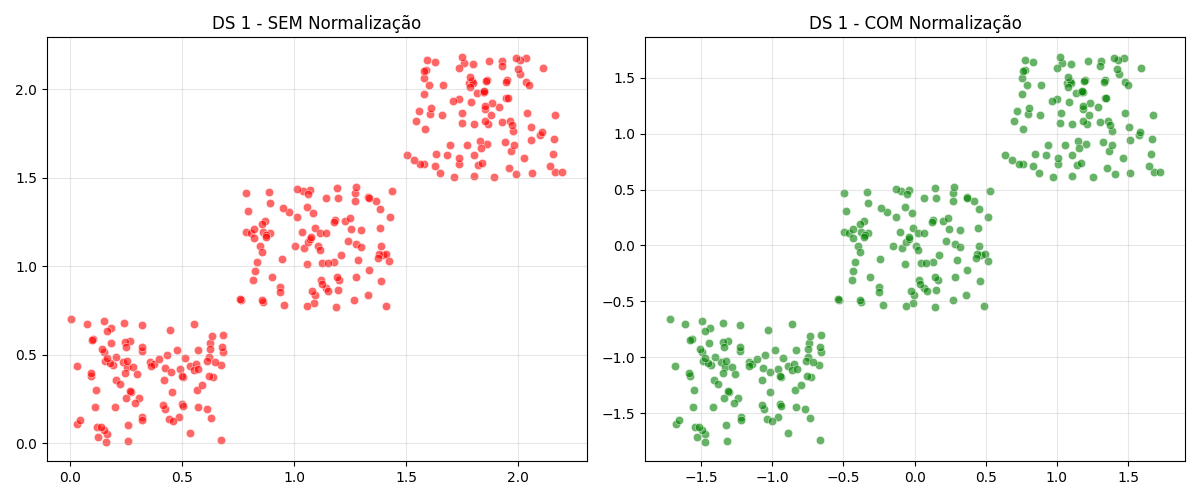
\includegraphics[width=\textwidth]{resultados/comparativo_normalizacao/comparacao_ds1.png}
\caption{DS1}
\end{subfigure}
\begin{subfigure}{0.48\textwidth}
\centering
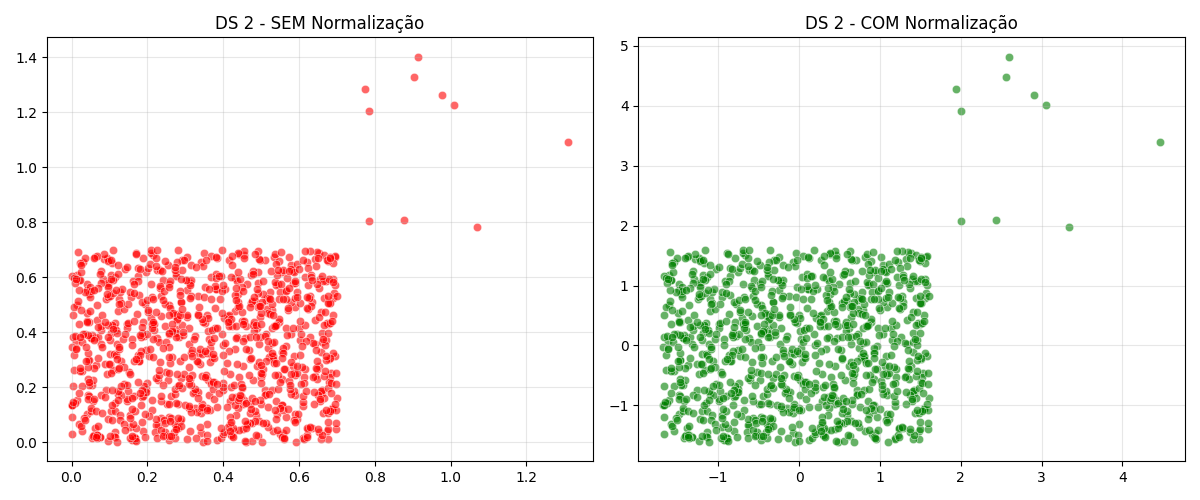
\includegraphics[width=\textwidth]{resultados/comparativo_normalizacao/comparacao_ds2.png}
\caption{DS2}
\end{subfigure}

\begin{subfigure}{0.48\textwidth}
\centering
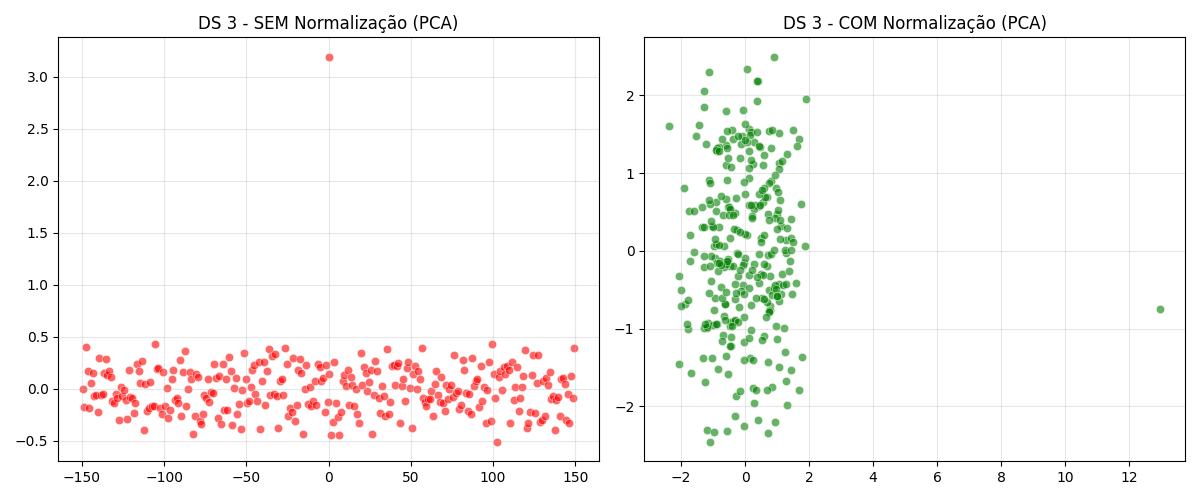
\includegraphics[width=\textwidth]{resultados/comparativo_normalizacao/comparacao_ds3.png}
\caption{DS3}
\end{subfigure}
\begin{subfigure}{0.48\textwidth}
\centering
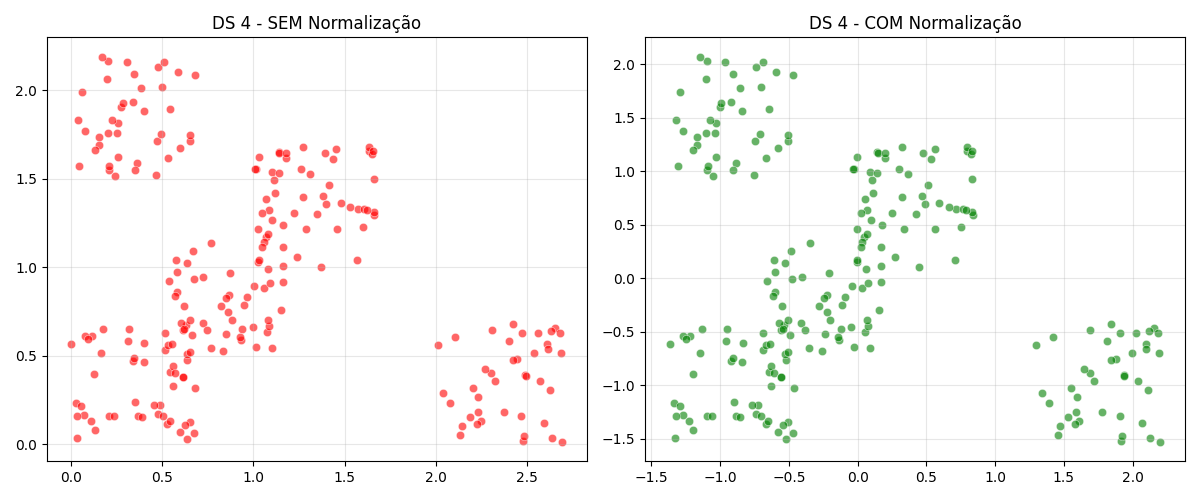
\includegraphics[width=\textwidth]{resultados/comparativo_normalizacao/comparacao_ds4.png}
\caption{DS4}
\end{subfigure}

\begin{subfigure}{0.55\textwidth}
\centering
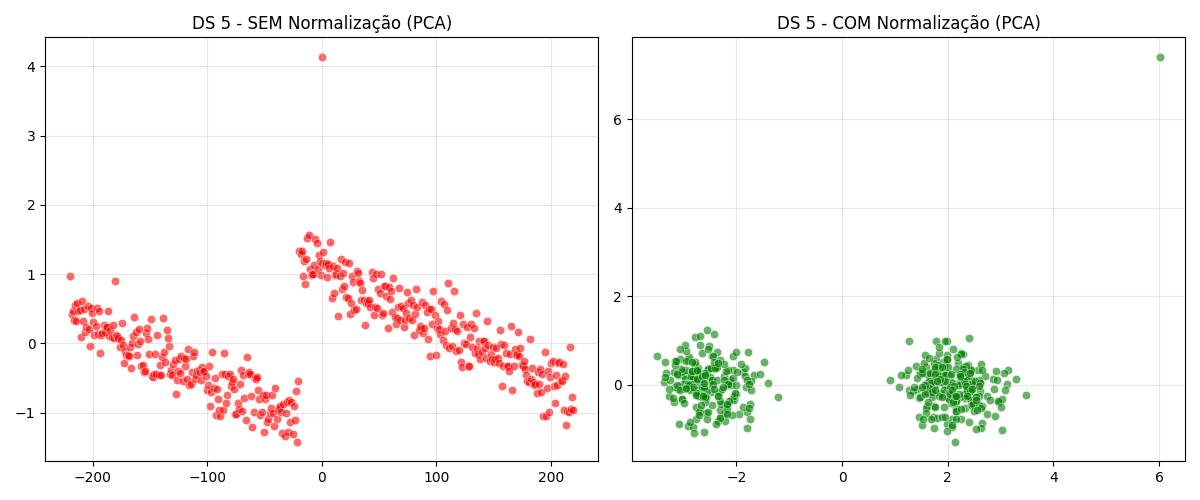
\includegraphics[width=\textwidth]{resultados/comparativo_normalizacao/comparacao_ds5.png}
\caption{DS5}
\end{subfigure}
\caption{Comparação visual antes e depois da normalização.}
\end{figure}

\section{Arquivos gerados}
Os principais arquivos gerados pelo projeto foram:
\begin{itemize}
    \item \texttt{datasets/DataSet1\_scaled.csv} a \texttt{datasets/DataSet5\_scaled.csv};
    \item \texttt{resultados/etapa1/}: gráficos exploratórios e resumo estatístico;
    \item \texttt{resultados/etapa3\_parametros/}: busca de parâmetros, rankings, CSVs e comparativos;
    \item \texttt{resultados/comparativo\_final/}: gráficos ClonalG vs k-Means e tabela final;
    \item \texttt{resultados/etapa4\_descoberta\_k/}: resultados da descoberta automática de \(k\).
\end{itemize}

\end{document}
